% ====================================================================================
\chapter{轨迹优化：让机器人优雅地运动}
% ====================================================================================

\section*{引言：火箭是怎么知道该怎么飞的？}

2015年12月21日，SpaceX的猎鹰9号火箭在发射后成功返回着陆——这是人类历史上第一次轨道级火箭的垂直回收。火箭在返回过程中需要精确控制发动机推力和姿态，才能稳稳降落在只有足球场大小的着陆平台上。
\storynote{Lev Pontryagin}{庞特里亚金（1908--1988），苏联数学家，14岁因煤油炉爆炸双目失明，靠母亲为他朗读论文完成研究。1955年他带领几位学生转向工程问题，为苏联空军研究"最短时间拦截"，1956年提出最大值原理——本章的伴随方程正是它的核心。}

\begin{figure}[htbp]
\centering
\begin{tikzpicture}[scale=0.8]
    % 火箭轨迹
    \draw[thick, blue, ->] (0, 6) to[out=-60, in=120] (2, 4) to[out=-60, in=150] (4, 2) to[out=-30, in=90] (5, 0);
    
    % 火箭（简化）
    \draw[fill=gray!30] (4.8, 0.5) -- (5, 1.5) -- (5.2, 0.5) -- cycle;
    \draw[fill=orange] (4.9, 0.3) -- (5, 0.5) -- (5.1, 0.3) -- cycle;
    
    % 着陆平台
    \fill[brown!50] (4, 0) rectangle (6, -0.2);
    \node at (5, -0.5) {\small 着陆平台};
    
    % 标注
    \node[blue] at (1, 5) {返回轨迹};
    \draw[->, red, thick] (4.5, 1.5) -- (4.5, 2.2);
    \node[red, right] at (4.5, 2) {\small 推力};
    
    % 问题
    \node[align=left] at (8, 3) {每一时刻该用\\多大推力？\\什么方向？};
\end{tikzpicture}
\caption{火箭返回着陆：一个复杂的轨迹优化问题}
\end{figure}

这就是\textbf{轨迹优化}问题：给定起点和终点，找到一条最优的运动轨迹，同时满足物理定律（动力学约束）。

令人惊喜的是，这个看似复杂的问题，其数学本质仍然是我们熟悉的\textbf{约束优化}——只不过约束变成了微分方程！

\vspace{0.3cm}
\noindent\textit{为什么火箭"知道"现在该用多大推力？为什么规划一条轨迹要从终点倒着算？为什么自动驾驶每隔零点几秒就把整个计划推翻重来一遍？}

\begin{quote}
\textbf{本章目标}：把"让一个系统从这里最优地走到那里"写成约束优化问题——目标是累计代价，约束是每个时刻都必须成立的动力学方程 $\dot{x} = f(x, u)$。你会看到，第1章的乘子 $\lambda$ 在这里变成一条随时间变化的曲线 $\lambda(t)$，它必须从终点往回算，这就是伴随方程；而"规划多步、只走一步、再重新规划"的 MPC，则是把这个优化问题塞进反馈回路里的工程做法。读完本章，你已经握住了第9章反向传播和第10章贝尔曼方程的钥匙。
\end{quote}

\begin{tcolorbox}[colback=yellow!10, colframe=orange!80, title=本章的核心观点]
\textbf{轨迹优化 = 变分法 + 拉格朗日乘子法。}本章的问题就是第1章的拉格朗日乘子法，只是约束从"一个方程 $g(x) = 0$"变成了"每个时刻一个方程 $\dot{x}(t) = f(x(t), u(t))$"，于是乘子从一个数 $\lambda$ 变成一个函数 $\lambda(t)$。

\begin{center}
\renewcommand{\arraystretch}{1.3}
\small
\begin{tabular}{lll}
\toprule
 & \textbf{第1章} & \textbf{本章} \\
\midrule
变量 & 向量 $x \in \R^n$ & 轨迹 $x(t)$ 与控制 $u(t)$ \\
目标 & $f(x)$ & $J = \int_0^T L(x, u)\,dt + \phi(x(T))$ \\
约束 & $g(x) = 0$ & $f(x, u) - \dot{x} = 0$（每个 $t$ 一条） \\
乘子 & $\lambda$（一个数） & $\lambda(t)$（协态，一条曲线） \\
拉格朗日函数 & $f + \lambda^\top g$ & $\int_0^T [L + \lambda^\top (f - \dot{x})]\,dt$ \\
一阶条件 & $\nabla f + \lambda^\top \nabla g = 0$，$g = 0$ & $\partial H/\partial u = 0$，$\dot{\lambda} = -\partial H/\partial x$，$\dot{x} = f$ \\
$\lambda$ 的意义 & 影子价格 & 未来代价对当前状态的敏感度 \\
\bottomrule
\end{tabular}
\end{center}
离散化之后（$x_{k+1} = f(x_k, u_k)$），这张表的右栏就变成第9章神经网络那张表的左栏。
\end{tcolorbox}

\begin{tcolorbox}[colback=green!5, colframe=green!60!black, title=学完这章，你将能够...]
\begin{itemize}
    \item 把"最省力移动物体"等问题写成最优控制形式
    \item 推导并求解简单系统的伴随方程
    \item 用直接法（离散化）数值求解轨迹优化问题
    \item 理解反向传播与伴随方法的数学联系
    \item 分析火箭着陆、机器人行走等实际案例
\end{itemize}
\end{tcolorbox}

% ------------------------------------------------------------------------------------
\section{从最简单的问题开始}

\subsection{问题：最省力地移动一个物体}

考虑一个质量为 $m$ 的物体在一维直线上运动。初始时刻 $t=0$ 在原点静止，我们要在时刻 $t=T$ 把它移动到位置 $x=1$，速度为零。

\begin{figure}[htbp]
\centering
\begin{tikzpicture}[scale=1.2]
    % 轨道
    \draw[thick] (-0.5, 0) -- (6, 0);
    
    % 起点
    \fill[blue] (0, 0) circle (3pt);
    \node[below] at (0, -0.2) {$x=0$};
    \node[above] at (0, 0.3) {$t=0$};
    \node[blue, above] at (0, 0.7) {静止};
    
    % 终点
    \fill[red] (5, 0) circle (3pt);
    \node[below] at (5, -0.2) {$x=1$};
    \node[above] at (5, 0.3) {$t=T$};
    \node[red, above] at (5, 0.7) {静止};
    
    % 物体和力
    \draw[fill=gray!30] (2.5, -0.2) rectangle (3, 0.2);
    \draw[->, thick, green!60!black] (3, 0) -- (4, 0);
    \node[green!60!black, above] at (3.5, 0) {$u(t)$};
    
    % 轨迹（虚线）
    \draw[dashed, blue] (0, 0.5) to[out=30, in=150] (5, 0.5);
\end{tikzpicture}
\caption{用最小的力把物体从起点移到终点}
\end{figure}

\textbf{物理定律}（牛顿第二定律）：
\[
m\ddot{x} = u(t)
\]

其中 $u(t)$ 是我们施加的力（控制输入）。

\textbf{边界条件}：
\begin{align}
x(0) &= 0, \quad \dot{x}(0) = 0 \quad \text{（初始：在原点静止）} \\
x(T) &= 1, \quad \dot{x}(T) = 0 \quad \text{（终止：在终点静止）}
\end{align}

\textbf{优化目标}：最小化总"能量消耗"（力的平方的积分）：
\[
J = \int_0^T \frac{1}{2} u(t)^2 \, dt
\]

为什么用 $u^2$ 而不是 $|u|$？因为平方可导，而且物理上电机的功率损耗与电流（力）的平方成正比。

\subsection{把问题写成标准形式}

为了方便，令 $m=1$，引入状态变量：
\[
x_1 = x \quad \text{（位置）}, \quad x_2 = \dot{x} \quad \text{（速度）}
\]

则动力学方程变成一阶系统：
\begin{align}
\dot{x}_1 &= x_2 \\
\dot{x}_2 &= u
\end{align}

\begin{keyformula}[title=轨迹优化的标准形式]
\begin{equation}
\min_{u(t)} \int_0^T L(x, u) \, dt
\end{equation}
\begin{align}
\text{s.t.} \quad & \dot{x} = f(x, u) \quad \text{（动力学约束）} \\
& x(0) = x_0, \quad x(T) = x_T \quad \text{（边界条件）}
\end{align}

在我们的例子中：
\begin{itemize}
    \item $x = (x_1, x_2)^\top$：状态向量
    \item $u$：控制输入
    \item $L(x, u) = \frac{1}{2}u^2$：瞬时代价
    \item $f(x, u) = (x_2, u)^\top$：动力学
\end{itemize}
\end{keyformula}

% ------------------------------------------------------------------------------------
\section{用拉格朗日乘子法处理动力学约束}

\subsection{关键思想}

回顾第1章：等式约束 $g(x) = 0$ 可以用拉格朗日乘子 $\lambda$ 处理。

现在的约束是微分方程 $\dot{x} = f(x, u)$，它必须在\textbf{每个时刻}都成立！
\review{第1章}{第1章的做法：每条等式约束 $g_i(x) = 0$ 配一个乘子 $\lambda_i$，写成 $\Lag = f + \sum_i \lambda_i g_i$，再对所有变量求导。这里的约束有无穷多条（每个时刻一条），所以乘子也有无穷多个——排成一个函数 $\lambda(t)$。}

所以我们需要\textbf{对每个时刻都引入一个乘子}——这就是连续时间的拉格朗日乘子 $\lambda(t)$。

\begin{insightbox}
\textbf{从有限维到无限维}：

有限维约束优化：$n$ 个约束 $\to$ $n$ 个乘子 $\lambda_1, \ldots, \lambda_n$

连续时间约束优化：每个时刻一个约束 $\to$ 乘子函数 $\lambda(t)$

乘子从"数"变成了"函数"！
\end{insightbox}
\review{第3章}{"乘子从数变成函数"在第3章已经发生过一次：离散化后每个 $y_{k+1} - y_k = v_k \Delta x$ 配一个 $\lambda_k$，取极限得到 $\lambda(x)$，而且 $\lambda_k = \partial F/\partial v_k$ 恰好是动量。本章只是把自变量从 $x$ 换成时间 $t$，把"斜率 $v$"换成"动力学 $f(x, u)$"。}

\subsection{构造哈密顿函数}

定义\textbf{哈密顿函数}（Hamiltonian）：

\begin{keyformula}[title=哈密顿函数]
\begin{equation}
H(x, u, \lambda) = L(x, u) + \lambda^\top f(x, u)
\end{equation}

在我们的例子中：
\begin{equation}
H = \frac{1}{2}u^2 + \lambda_1 x_2 + \lambda_2 u
\end{equation}
\end{keyformula}

\textbf{为什么叫哈密顿函数？}

这和分析力学中的哈密顿量有深刻的联系！第5章的哈密顿量是 $H = p\dot{q} - L$（保守系统里等于 $T + V$）；这里的 $H = L + \lambda^\top \dot{x}$ 来自同一个勒让德变换：把 $\lambda$ 看成动量 $p$，两者只差 $L$ 前面的符号（一个求最小作用量，一个求最小代价）。
\review{第5章}{第5章：$H = \sum_i \dot{q}_i \,\partial L/\partial \dot{q}_i - L$，不显含 $t$ 时守恒。这里的 $\lambda$ 扮演 $\partial L/\partial \dot{q}$（动量）的角色——第3章已经证明过"乘子 = 动量"。}

\subsection{增广的目标函数}

把约束"吸收"到目标函数中：

\begin{align}
J_{aug} &= \int_0^T \left[ L(x, u) + \lambda^\top (f(x, u) - \dot{x}) \right] dt \\
&= \int_0^T \left[ L(x, u) + \lambda^\top f(x, u) - \lambda^\top \dot{x} \right] dt
\end{align}

注意最后那项 $\lambda^\top \dot{x}$，对它用分部积分：
\clarify{为什么把约束写成 $f - \dot{x}$ 而不是 $\dot{x} - f$？两种写法只差 $\lambda$ 的符号。写成 $f - \dot{x}$ 时，推出来的 $\lambda$ 恰好是"未来代价对当前状态的梯度"，符号最顺手；这是最优控制文献的惯例。}

\[
\int_0^T \lambda^\top \dot{x} \, dt = [\lambda^\top x]_0^T - \int_0^T \dot{\lambda}^\top x \, dt
\]

代入得：
\begin{equation}
J_{aug} = -\lambda(T)^\top x(T) + \lambda(0)^\top x(0) + \int_0^T \left[ \underbrace{L + \lambda^\top f}_{H} + \dot{\lambda}^\top x \right] dt
\end{equation}

\subsection{变分条件}

现在对 $x(t)$、$u(t)$、$\lambda(t)$ 分别变分，要求 $J_{aug}$ 取极值。

\paragraph{对 $u$ 变分}（最优性条件）

\[
\frac{\partial H}{\partial u} = 0
\]

在我们的例子中：$\frac{\partial H}{\partial u} = u + \lambda_2 = 0$，即 $u = -\lambda_2$。

\paragraph{对 $x$ 变分}（伴随方程/协态方程）

\[
\dot{\lambda} = -\frac{\partial H}{\partial x}
\]

\begin{insightbox}
\textbf{伴随方程的直觉}：为什么要"向后"传播？

想象你在规划一次旅行。你的决定（控制$u$）会影响后续所有行程（状态$x$）。那么，\textbf{某一天的选择有多重要}，取决于它对\textbf{后面所有日子}的影响。

伴随变量 $\lambda(t)$ 正是量化这种"未来影响"的工具：
\begin{itemize}
    \item $\lambda(t)$ = "时刻$t$的状态变化对\textbf{未来总代价}的影响"
    \item 必须从终点往回算（因为要先知道终点代价，才能算中间点的影响）
    \item 这和第9章神经网络的\textbf{反向传播}是同一个思想！
\end{itemize}

\textbf{一句话总结}：伴随方程告诉我们"当前选择对未来的影响有多大"，所以必须从未来往回算。
\end{insightbox}

在我们的例子中：
\begin{align}
\dot{\lambda}_1 &= -\frac{\partial H}{\partial x_1} = 0 \\
\dot{\lambda}_2 &= -\frac{\partial H}{\partial x_2} = -\lambda_1
\end{align}

\paragraph{对 $\lambda$ 变分}（状态方程）

\[
\dot{x} = \frac{\partial H}{\partial \lambda} = f(x, u)
\]

这就是原来的动力学约束！

\begin{keytheorem}[title=Pontryagin 最大值原理（简化版）]
最优轨迹 $(x^*(t), u^*(t))$ 和对应的乘子 $\lambda^*(t)$ 满足：

\begin{enumerate}
    \item \textbf{状态方程}（向前积分）：
    \[
    \dot{x} = \frac{\partial H}{\partial \lambda} = f(x, u)
    \]
    
    \item \textbf{伴随方程}（向后积分）：
    \[
    \dot{\lambda} = -\frac{\partial H}{\partial x}
    \]
    
    \item \textbf{最优性条件}：
    \[
    \frac{\partial H}{\partial u} = 0
    \]
\end{enumerate}
\end{keytheorem}
\preview{这三条方程第9章会原样出现：把"时刻 $t$"换成"第 $i$ 层"，$x$ 换成层输出 $z_i$，$u$ 换成权重 $\theta_i$，伴随方程就叫"反向传播"；第10章再把 $\lambda$ 换成值函数的梯度，伴随方程就变成贝尔曼方程。}

\begin{physicalmeaning}
$\lambda(t)$ 的物理意义：\textbf{未来总代价对当前状态的敏感度}。

$\lambda_i(t) = \frac{\partial J^*}{\partial x_i(t)}$ 告诉我们：如果在时刻 $t$ 把状态 $x_i$ 增加一点点，未来的总代价会增加多少。

这就像股票的"影子价格"——当前持有的价值取决于未来的收益。
\end{physicalmeaning}
\clarify{符号约定提醒：本书动态各章统一把动力学约束写成"$f - \dot{x}$"（离散版 $f(x_k,u_k) - x_{k+1}$）的形式，于是 $\lambda$ 总是"最优代价对状态的梯度"：本章连续与离散部分、第9章的反向传播、第10章的值函数梯度、第11章的时间反传都是如此。第1章的规则 $\lambda = -df^*/d\epsilon$ 依然成立——把约束放松成 $f - \dot{x} = \epsilon$ 相当于把状态"往回拨"$\epsilon$，对状态的梯度前面因此多出一个负号，两者正好抵消。若像某些教材那样把约束写成 $\dot{x} - f$，推出的 $\lambda$ 只差一个整体负号，判断口径只看一条："$\lambda$ 是不是代价对状态的梯度"。}

% ------------------------------------------------------------------------------------
\section{完整求解：最省力移动问题}

现在让我们完整求解前面的问题。

\subsection{第一步：写出所有方程}

\textbf{状态方程}：
\begin{align}
\dot{x}_1 &= x_2 \\
\dot{x}_2 &= u
\end{align}

\textbf{伴随方程}：
\begin{align}
\dot{\lambda}_1 &= 0 \\
\dot{\lambda}_2 &= -\lambda_1
\end{align}

\textbf{最优性条件}：
\[
u = -\lambda_2
\]

\textbf{边界条件}：
\begin{align}
x_1(0) = 0, \quad x_2(0) = 0 \quad &\text{（初始条件）} \\
x_1(T) = 1, \quad x_2(T) = 0 \quad &\text{（终端条件）}
\end{align}

\subsection{第二步：解伴随方程}

从 $\dot{\lambda}_1 = 0$ 得：
\[
\lambda_1(t) = c_1 \quad \text{（常数）}
\]

从 $\dot{\lambda}_2 = -\lambda_1 = -c_1$ 得：
\[
\lambda_2(t) = -c_1 t + c_2
\]

\subsection{第三步：得到最优控制}

由最优性条件 $u = -\lambda_2$：
\[
u^*(t) = c_1 t - c_2
\]

最优控制是\textbf{时间的线性函数}！

\subsection{第四步：解状态方程}

把 $u^* = c_1 t - c_2$ 代入状态方程。

从 $\dot{x}_2 = u$ 积分：
\[
x_2(t) = \int_0^t u \, d\tau = \int_0^t (c_1 \tau - c_2) d\tau = \frac{c_1 t^2}{2} - c_2 t + x_2(0)
\]

由 $x_2(0) = 0$：
\[
x_2(t) = \frac{c_1 t^2}{2} - c_2 t
\]

从 $\dot{x}_1 = x_2$ 积分：
\[
x_1(t) = \int_0^t x_2 \, d\tau = \int_0^t \left(\frac{c_1 \tau^2}{2} - c_2 \tau\right) d\tau = \frac{c_1 t^3}{6} - \frac{c_2 t^2}{2}
\]

\subsection{第五步：确定常数}

用终端条件 $x_1(T) = 1$ 和 $x_2(T) = 0$：

从 $x_2(T) = 0$：
\[
\frac{c_1 T^2}{2} - c_2 T = 0 \quad \Rightarrow \quad c_2 = \frac{c_1 T}{2}
\]

从 $x_1(T) = 1$：
\[
\frac{c_1 T^3}{6} - \frac{c_2 T^2}{2} = 1
\]

把 $c_2 = \frac{c_1 T}{2}$ 代入：
\[
\frac{c_1 T^3}{6} - \frac{c_1 T}{2} \cdot \frac{T^2}{2} = \frac{c_1 T^3}{6} - \frac{c_1 T^3}{4} = -\frac{c_1 T^3}{12} = 1
\]

解得：
\[
c_1 = -\frac{12}{T^3}, \quad c_2 = \frac{c_1 T}{2} = -\frac{6}{T^2}
\]

\subsection{第六步：写出最终解}

\begin{keyformula}[title=最优解]
\textbf{最优控制}：
\begin{equation}
u^*(t) = c_1 t - c_2 = -\frac{12}{T^3} t + \frac{6}{T^2} = \frac{6}{T^2}\left(1 - \frac{2t}{T}\right)
\end{equation}

\textbf{最优轨迹}：
\begin{equation}
x_1^*(t) = \frac{c_1 t^3}{6} - \frac{c_2 t^2}{2} = -\frac{2t^3}{T^3} + \frac{3t^2}{T^2} = \left(\frac{t}{T}\right)^2 \left(3 - \frac{2t}{T}\right)
\end{equation}
\end{keyformula}

\subsection{验证与可视化}

取 $T = 1$，画出最优解：

\begin{figure}[htbp]
\centering
\begin{tikzpicture}[scale=0.85]
    % 位置图
    \begin{scope}
        \draw[->] (0, 0) -- (4.2, 0) node[right] {$t$};
        \draw[->] (0, 0) -- (0, 2.5) node[above] {$x_1$};

        % 刻度
        \node[below] at (3.8, 0) {$T$};
        \node[left] at (0, 2) {$1$};
        \draw (3.8, 0.05) -- (3.8, -0.05);
        \draw (0.05, 2) -- (-0.05, 2);

        % 轨迹 x(t) = 3t^2 - 2t^3 (T=1时)
        \draw[thick, blue, domain=0:3.8, samples=50] plot (\x, {2*(3*(\x/3.8)^2 - 2*(\x/3.8)^3)});

        \node[blue] at (1.9, 2.3) {位置 $x_1(t)$};
    \end{scope}

    % 速度图
    \begin{scope}[xshift=5.5cm]
        \draw[->] (0, -0.5) -- (4.2, -0.5) node[right] {$t$};
        \draw[->] (0, -0.5) -- (0, 2) node[above] {$x_2$};

        % 刻度
        \node[below] at (3.8, -0.5) {$T$};
        \node[below] at (1.9, -0.5) {$T/2$};

        % 速度 v(t) = 6t - 6t^2 (T=1时)
        \draw[thick, green!60!black, domain=0:3.8, samples=50] plot (\x, {1.5*(6*(\x/3.8)/3.8 - 6*(\x/3.8)^2/3.8) - 0.5});

        \node[green!60!black] at (1.9, 1.8) {速度 $x_2(t)$};
    \end{scope}

    % 控制图
    \begin{scope}[xshift=11cm]
        \draw[->] (0, -1) -- (4.2, -1) node[right] {$t$};
        \draw[->] (0, -1.5) -- (0, 2) node[above] {$u$};

        % 刻度
        \node[below] at (3.8, -1) {$T$};

        % 控制 u(t) = 6 - 12t (T=1时)
        \draw[thick, red, domain=0:3.8] plot (\x, {0.3*(6 - 12*\x/3.8) - 1});

        % 零线
        \draw[dashed, gray] (0, -1) -- (3.8, -1);

        \node[red] at (1.9, 1.5) {控制 $u(t)$};
    \end{scope}
\end{tikzpicture}
\caption{最优解的三个分量：位置平滑过渡，速度先增后减，控制力从正变负}
\end{figure}

\textbf{物理解释}：

\begin{itemize}
    \item \textbf{前半段}（$t < T/2$）：$u > 0$，向右推，加速
    \item \textbf{后半段}（$t > T/2$）：$u < 0$，向左推，减速
    \item \textbf{中点}（$t = T/2$）：速度最大，控制力过零
    \item \textbf{终点}（$t = T$）：恰好停在目标位置
\end{itemize}

这就是"最优"的直觉含义：不多不少，刚刚好！

\begin{insightbox}
\textbf{为什么最优控制是线性的？}

这是因为我们的系统是\textbf{线性的}（$\ddot{x} = u$），代价是\textbf{二次的}（$\int u^2 dt$）。

线性系统 + 二次代价 $\Rightarrow$ 最优控制 $u^*(t)$ 是时间的线性函数

严格地说，本例（终端固定、无状态代价）叫\textbf{最小能量控制}。加上状态的二次代价之后，就是控制工程中极其重要的\textbf{线性二次调节器}（LQR）——那时"线性"指的是最优控制是状态的线性反馈 $u = -Kx$。
\end{insightbox}

图~\ref{fig:chap08_minimum_effort} 画出了这个解析解，并展示了时间越长、所需控制能量越小的规律。

\begin{figure}[htbp]
\centering
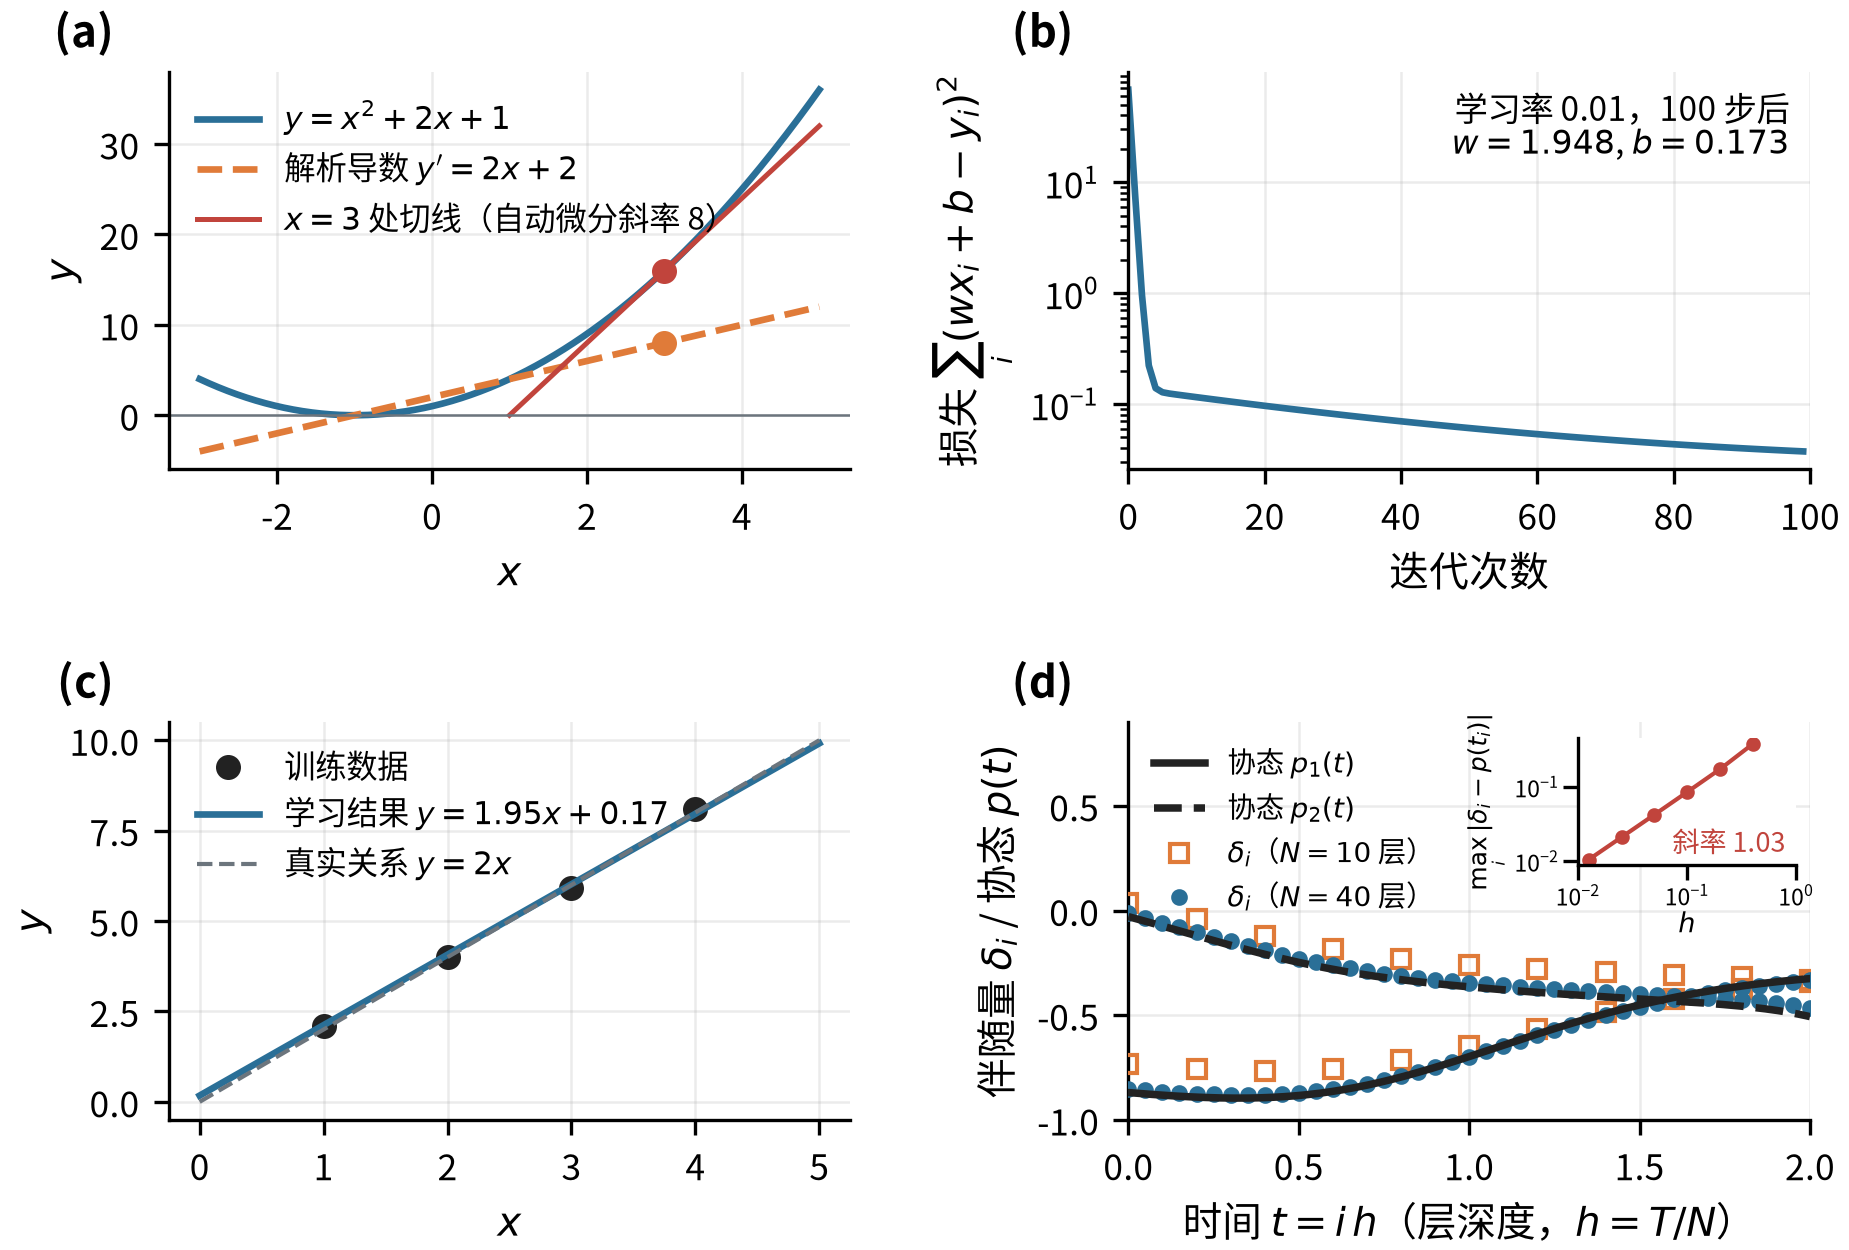
\includegraphics[width=0.95\textwidth]{figs_chap08/chap08_fig1.png}
\caption{最省力移动问题的解析解可视化。左图：最优轨迹$x^*(t) = (t/T)^2(3 - 2t/T)$（位置）和速度曲线——先加速后减速，在中点速度最大；中图：最优控制$u^*(t) = 6/T^2(1 - 2t/T)$——前半段加速（$u > 0$），后半段减速（$u < 0$）；右图：能量消耗随时间长度 $T$ 的关系——时间越长，所需控制能量越小，符合"慢工出细活"的直觉。}
\label{fig:chap08_minimum_effort}
\end{figure}

% ------------------------------------------------------------------------------------
\section{离散时间的视角}

实际计算机控制时，我们不能处理连续时间，必须离散化。这反而让问题变得更清晰！

\subsection{离散化}

把时间 $[0, T]$ 分成 $N$ 段，每段长度 $\Delta t = T/N$。

时刻：$t_k = k \cdot \Delta t$，$k = 0, 1, \ldots, N$

\textbf{离散状态和控制}：
\begin{itemize}
    \item $x_k \approx x(t_k)$：第 $k$ 时刻的状态
    \item $u_k \approx u(t_k)$：第 $k$ 时刻的控制
\end{itemize}

\textbf{离散动力学}（欧拉法）：
\[
x_{k+1} = x_k + \Delta t \cdot f(x_k, u_k)
\]

\textbf{离散代价}：
\[
J = \sum_{k=0}^{N-1} L(x_k, u_k) \cdot \Delta t
\]

\subsection{变成有限维优化问题}

\begin{keyformula}[title=离散轨迹优化]
\begin{equation}
\min_{x_0, u_0, x_1, u_1, \ldots, x_N, u_{N-1}} \sum_{k=0}^{N-1} L(x_k, u_k)
\end{equation}
\begin{align}
\text{s.t.} \quad & x_{k+1} = x_k + \Delta t \cdot f(x_k, u_k), \quad k = 0, \ldots, N-1 \\
& x_0 = x_{init} \\
& x_N = x_{target}
\end{align}
\end{keyformula}

这是一个\textbf{有限维的等式约束优化问题}！可以直接用拉格朗日乘子法。

\subsection{例子：一阶系统，$N = 2$}

考虑一阶系统 $\dot{x} = u$，从 $x(0) = 0$ 到 $x(T) = 1$。

离散化（$N=2$，$\Delta t = T/2$）：
\begin{align}
x_1 &= x_0 + \Delta t \cdot u_0 = \frac{T}{2} u_0 \\
x_2 &= x_1 + \Delta t \cdot u_1 = x_1 + \frac{T}{2} u_1
\end{align}

边界条件：$x_0 = 0$，$x_2 = 1$。

从第一个方程：$x_1 = \frac{T}{2} u_0$

代入第二个方程：$1 = \frac{T}{2} u_0 + \frac{T}{2} u_1$，即 $u_0 + u_1 = \frac{2}{T}$

\textbf{优化问题}：
\[
\min_{u_0, u_1} \frac{1}{2}u_0^2 + \frac{1}{2}u_1^2 \quad \text{s.t.} \quad u_0 + u_1 = \frac{2}{T}
\]

\textbf{用拉格朗日乘子法}：
\[
\mathcal{L} = \frac{1}{2}u_0^2 + \frac{1}{2}u_1^2 + \lambda\left(u_0 + u_1 - \frac{2}{T}\right)
\]

一阶条件：
\begin{align}
\frac{\partial \mathcal{L}}{\partial u_0} &= u_0 + \lambda = 0 \quad \Rightarrow \quad u_0 = -\lambda \\
\frac{\partial \mathcal{L}}{\partial u_1} &= u_1 + \lambda = 0 \quad \Rightarrow \quad u_1 = -\lambda \\
\frac{\partial \mathcal{L}}{\partial \lambda} &= u_0 + u_1 - \frac{2}{T} = 0
\end{align}

从前两个方程：$u_0 = u_1$

代入第三个方程：$2u_0 = \frac{2}{T}$，所以 $u_0 = u_1 = \frac{1}{T}$

\textbf{最优解}：匀速运动！$u_0 = u_1 = \frac{1}{T}$

这与连续时间的解一致（对于一阶系统，最省力的方法就是匀速）。这种"先离散化、再当成普通约束优化来解"的做法叫\textbf{直接法}。
\tryit{把 $N$ 改成 4、8、16，用 \texttt{scipy.optimize.minimize} 加等式约束求解，看 $u_k$ 是否始终等于 $1/T$。再把系统换回二阶的 $\ddot{x} = u$（状态取 $(x, v)$），看数值解如何逼近前面的解析解 $u^*(t) = \frac{6}{T^2}(1 - \frac{2t}{T})$。这就是"直接法"。}

% ------------------------------------------------------------------------------------
\section{伴随方程：反向传播的原型}

这一节我们来仔细推导离散时间的伴随方程，你会发现它和神经网络的反向传播\textbf{完全一样}！

\subsection{离散轨迹优化问题}

先把问题写清楚。我们要解决：

\begin{equation}
\min_{u_0, u_1, \ldots, u_{N-1}} J = \sum_{k=0}^{N-1} L_k(x_k, u_k) + \phi(x_N)
\end{equation}

约束是离散动力学：
\begin{equation}
x_{k+1} = f(x_k, u_k), \quad k = 0, 1, \ldots, N-1
\end{equation}

初始条件 $x_0$ 给定。

\textbf{决策变量}：控制序列 $u_0, u_1, \ldots, u_{N-1}$

\textbf{注意}：状态 $x_1, x_2, \ldots, x_N$ 不是独立的决策变量！一旦给定 $u_0, \ldots, u_{N-1}$，状态就由动力学唯一确定了。

\subsection{用拉格朗日乘子处理动力学约束}

虽然状态由控制决定，但直接计算 $\frac{\partial J}{\partial u_k}$ 很麻烦（因为 $u_k$ 通过动力学影响后面所有的状态）。

聪明的做法：把状态也当作独立变量，用拉格朗日乘子处理动力学约束。

\textbf{构造拉格朗日函数}：

对每个动力学约束 $f(x_k, u_k) - x_{k+1} = 0$（与连续部分的 $f - \dot{x}$ 同一写法），引入乘子 $\lambda_{k+1}$：

\begin{equation}
\mathcal{L} = \underbrace{\sum_{k=0}^{N-1} L_k(x_k, u_k) + \phi(x_N)}_{\text{原目标函数}} + \underbrace{\sum_{k=0}^{N-1} \lambda_{k+1}^\top \left[ f(x_k, u_k) - x_{k+1} \right]}_{\text{约束项（应该=0）}}
\end{equation}

展开写得更清楚：
\begin{align}
\mathcal{L} &= L_0(x_0, u_0) + \lambda_1^\top [f(x_0, u_0) - x_1] \\
&+ L_1(x_1, u_1) + \lambda_2^\top [f(x_1, u_1) - x_2] \\
&+ L_2(x_2, u_2) + \lambda_3^\top [f(x_2, u_2) - x_3] \\
&+ \cdots \\
&+ L_{N-1}(x_{N-1}, u_{N-1}) + \lambda_N^\top [f(x_{N-1}, u_{N-1}) - x_N] \\
&+ \phi(x_N)
\end{align}

\subsection{对各变量求偏导}

现在对 $\mathcal{L}$ 分别对 $x_k$、$u_k$、$\lambda_k$ 求偏导，令其为零。

\paragraph{对 $\lambda_{k+1}$ 求导}（恢复动力学约束）

\[
\frac{\partial \mathcal{L}}{\partial \lambda_{k+1}} = f(x_k, u_k) - x_{k+1} = 0
\]

这就是原来的动力学方程！没有新信息。

\paragraph{对 $u_k$ 求导}（最优性条件）

$u_k$ 只出现在 $L_k(x_k, u_k)$ 和 $f(x_k, u_k)$ 中：

\[
\frac{\partial \mathcal{L}}{\partial u_k} = \frac{\partial L_k}{\partial u_k} + \lambda_{k+1}^\top \frac{\partial f}{\partial u_k} = 0
\]

像连续部分那样定义离散哈密顿量 $H_k = L_k(x_k, u_k) + \lambda_{k+1}^\top f(x_k, u_k)$，这个条件就是：
\begin{equation}
\boxed{\frac{\partial H_k}{\partial u_k} = \frac{\partial L_k}{\partial u_k} + \lambda_{k+1}^\top \frac{\partial f}{\partial u_k} = 0}
\end{equation}

这告诉我们：最优控制时，代价对 $u_k$ 的"直接"敏感度，与"经由下一步状态传回来"的敏感度（乘子 × 动力学对 $u_k$ 的敏感度）恰好抵消。

\paragraph{对 $x_k$（$k = 1, \ldots, N-1$）求导}（伴随方程）

这是最关键的一步！让我们仔细看 $x_k$ 出现在哪里：

\begin{itemize}
    \item $L_k(x_k, u_k)$ 中：贡献 $\frac{\partial L_k}{\partial x_k}$
    \item $\lambda_{k+1}^\top [f(x_k, u_k) - x_{k+1}]$ 中的 $f(x_k, u_k)$：贡献 $\lambda_{k+1}^\top \frac{\partial f}{\partial x_k}$
    \item $\lambda_k^\top [f(x_{k-1}, u_{k-1}) - x_k]$ 中的 $-x_k$：贡献 $-\lambda_k^\top$
\end{itemize}

令偏导为零：
\[
\frac{\partial \mathcal{L}}{\partial x_k} = \frac{\partial L_k}{\partial x_k} - \lambda_k^\top + \lambda_{k+1}^\top \frac{\partial f}{\partial x_k} = 0
\]

整理得到\textbf{伴随方程}：
\begin{equation}
\boxed{\lambda_k = \left(\frac{\partial f}{\partial x_k}\right)^\top \lambda_{k+1} + \frac{\partial L_k}{\partial x_k}^\top = \frac{\partial H_k}{\partial x_k}^\top}
\end{equation}

\paragraph{对 $x_N$ 求导}（终端条件）

$x_N$ 出现在 $\phi(x_N)$ 和 $-\lambda_N^\top x_N$ 中：
\[
\frac{\partial \mathcal{L}}{\partial x_N} = \frac{\partial \phi}{\partial x_N} - \lambda_N^\top = 0
\]

得到\textbf{终端条件}：
\begin{equation}
\boxed{\lambda_N = \frac{\partial \phi}{\partial x_N}^\top}
\end{equation}
\think{$\lambda_N = \partial \phi/\partial x_N$ 说的是"终点状态挪一点，终端代价变多少"——正是影子价格。它和第1章的 $\lambda = -df^*/d\epsilon$ 差一个负号，矛盾吗？（提示：把最后一条约束放松成 $f(x_{N-1}, u_{N-1}) - x_N = \epsilon$，意味着 $x_N$ 减少 $\epsilon$，于是 $dJ^*/d\epsilon = -\partial\phi/\partial x_N = -\lambda_N$，第1章的规则原封不动。）}

\subsection{具体例子：手算伴随方程}

让我们用一个超级简单的例子来验证这些公式。

\textbf{问题}：一维系统，$N = 2$ 步

\begin{itemize}
    \item 动力学：$x_{k+1} = x_k + u_k$（离散积分器）
    \item 代价：$J = u_0^2 + u_1^2 + 10 x_2^2$（最小化控制能量，同时让终点尽量接近零）
    \item 初始条件：$x_0 = 1$
\end{itemize}


\textbf{第一步：前向传播}

\begin{align}
x_1 &= x_0 + u_0 = 1 + u_0 \\
x_2 &= x_1 + u_1 = 1 + u_0 + u_1
\end{align}

\textbf{第二步：计算各偏导数}

动力学 $f(x, u) = x + u$：
\[
\frac{\partial f}{\partial x} = 1, \quad \frac{\partial f}{\partial u} = 1
\]

代价 $L_k = u_k^2$：
\[
\frac{\partial L_k}{\partial x} = 0, \quad \frac{\partial L_k}{\partial u} = 2u_k
\]

终端代价 $\phi = 10 x_2^2$：
\[
\frac{\partial \phi}{\partial x_2} = 20 x_2
\]

\textbf{第三步：后向传播}（计算伴随变量）

终端条件：
\[
\lambda_2 = \frac{\partial \phi}{\partial x_2} = 20 x_2 = 20(1 + u_0 + u_1)
\]

伴随方程（$k = 1$）：
\[
\lambda_1 = \frac{\partial f}{\partial x}^\top \lambda_2 + \frac{\partial L_1}{\partial x}^\top = 1 \cdot \lambda_2 + 0 = \lambda_2 = 20(1 + u_0 + u_1)
\]

\textbf{第四步：最优性条件}

对 $u_1$：
\[
\frac{\partial L_1}{\partial u_1} + \lambda_2 \cdot \frac{\partial f}{\partial u} = 0 \quad \Rightarrow \quad 2u_1 = -\lambda_2 \cdot 1 = -20(1 + u_0 + u_1)
\]

整理：$2u_1 + 20u_1 = -20 - 20u_0$，即 $22u_1 = -20 - 20u_0$

对 $u_0$：
\[
\frac{\partial L_0}{\partial u_0} + \lambda_1 \cdot \frac{\partial f}{\partial u} = 0 \quad \Rightarrow \quad 2u_0 = -\lambda_1 \cdot 1 = -20(1 + u_0 + u_1)
\]

整理：$2u_0 + 20u_0 = -20 - 20u_1$，即 $22u_0 = -20 - 20u_1$

\textbf{第五步：解方程组}

\begin{align}
22u_0 &= -20 - 20u_1 \\
22u_1 &= -20 - 20u_0
\end{align}

两式相减：$22(u_0 - u_1) = -20(u_1 - u_0) = 20(u_0 - u_1)$

所以 $2(u_0 - u_1) = 0$，即 $u_0 = u_1$。

代入第一个方程：$22u_0 = -20 - 20u_0$，得 $42u_0 = -20$，即：
\[
u_0 = u_1 = -\frac{20}{42} = -\frac{10}{21} \approx -0.476
\]

\textbf{验证}：
\begin{align}
x_1 &= 1 + u_0 = 1 - 0.476 = 0.524 \\
x_2 &= x_1 + u_1 = 0.524 - 0.476 = 0.048
\end{align}

终点 $x_2 \approx 0.048$，接近零！

代价：$J = u_0^2 + u_1^2 + 10x_2^2 = 0.227 + 0.227 + 0.023 = 0.477$

\begin{insightbox}
\textbf{我们刚才做了什么？}

\begin{enumerate}
    \item 把优化问题写成拉格朗日函数
    \item 对各变量求导，得到\textbf{伴随方程}
    \item \textbf{前向}计算状态，\textbf{后向}计算伴随变量
    \item 用最优性条件求解最优控制
\end{enumerate}

\end{insightbox}


% ------------------------------------------------------------------------------------
\section{模型预测控制（MPC）}

\subsection{为什么需要 MPC？}

到目前为止，我们假设：
\begin{itemize}
    \item 模型完全准确（动力学 $f$ 精确已知）
    \item 没有外部干扰（没有风、没有摩擦变化）
    \item 可以一次性规划整个轨迹（从头到尾）
\end{itemize}

但现实世界不是这样的！

\begin{figure}[htbp]
\centering
\begin{tikzpicture}[scale=0.9]
    % 理想情况
    \begin{scope}
        \node[font=\bfseries] at (2, 2.5) {理想情况};
        \draw[thick] (0, 0) -- (4, 0);
        \draw[blue, thick, ->] (0.5, 0.3) to[out=30, in=150] (3.5, 0.3);
        \fill[blue] (0.5, 0.3) circle (2pt);
        \fill[red] (3.5, 0.3) circle (2pt);
        \node at (2, -0.5) {\small 规划一次，完美执行};
    \end{scope}
    
    % 现实情况
    \begin{scope}[xshift=6cm]
        \node[font=\bfseries] at (2, 2.5) {现实情况};
        \draw[thick] (0, 0) -- (4, 0);
        \draw[blue, thick, ->] (0.5, 0.3) to[out=30, in=180] (1.5, 0.8);
        \draw[blue, thick, dashed] (1.5, 0.8) to[out=0, in=150] (3.5, 0.3);
        \draw[red, thick, ->] (1.5, 0.8) to[out=-30, in=180] (2.2, 0.2);
        \fill[blue] (0.5, 0.3) circle (2pt);
        \fill[red] (3.5, 0.3) circle (2pt);
        
        % 干扰
        \draw[->, thick, orange] (1.3, 1.5) -- (1.5, 0.9);
        \node[orange] at (1.3, 1.8) {\small 干扰！};
        
        \node at (2, -0.5) {\small 计划被打乱};
    \end{scope}
\end{tikzpicture}
\caption{理想 vs 现实：干扰会打乱预先规划好的轨迹}
\end{figure}

\textbf{具体例子}：

\begin{itemize}
    \item \textbf{模型误差}：你以为摩擦系数是 0.5，实际是 0.3（路面结冰了）
    \item \textbf{外部干扰}：无人机在飞行中突然遇到侧风
    \item \textbf{环境变化}：自动驾驶车前方突然出现行人
\end{itemize}

如果我们在起点规划好整条轨迹然后"闭着眼执行"，一点小扰动就会让系统偏离目标！

\textbf{MPC 的哲学}：\textbf{计划赶不上变化，所以我们边走边规划}！
\think{MPC 每一步都重新解优化问题，那上一步算出的乘子 $\lambda$ 还有用吗？提示：$\lambda$ 是"未来代价对当前状态的敏感度"，而当前状态刚刚被测量更新了。第10章的值函数会给出更系统的答案：它就是"把 $\lambda$ 对所有可能的当前状态预先算好"。}

\subsection{MPC 的核心思想}

\begin{keyformula}[title=MPC 框架]
在\textbf{每个}时刻 $t$：
\begin{enumerate}
    \item \textbf{测量}：获取当前真实状态 $x_t$（通过传感器）
    \item \textbf{规划}：以 $x_t$ 为起点，求解未来 $N$ 步的轨迹优化问题
    \item \textbf{执行}：只执行优化结果的\textbf{第一步}控制 $u_t^*$
    \item \textbf{重复}：下一时刻回到第1步，用新测量的状态重新规划
\end{enumerate}
\end{keyformula}

\begin{figure}[htbp]
\centering
\begin{tikzpicture}[scale=1.0]

    % 时间轴
    \draw[->] (0,0) -- (17,0) node[right] {时间};

    % --------------------------
    % t=0 时刻
    % --------------------------
    \begin{scope}[xshift=0cm]
        \node[above] at (1,2.2) {\small $t=0$};
        \draw[thick] (1,0.1) -- (1,-0.1);

        % 预测轨迹
        \draw[blue, thick] (1,1.4) -- (2,1.6) -- (3,1.5) -- (4,1.3) -- (5,1.1);
        \foreach \x in {1,2,3,4,5} {
            \fill[blue] (\x, {1.4 + 0.2*sin((\x-1)*40)}) circle (2pt);
        }

        \node[blue, above] at (3,1.8) {\small 规划 $N=4$ 步};

        % 执行一步
        \draw[red, ultra thick] (1,0) -- (2,0);
        \draw[red, ultra thick, ->] (1,1.4) -- (2,1.6);
        \node[red, below] at (1.5,-0.3) {\small 执行};
    \end{scope}

    % --------------------------
    % t=1 时刻
    % --------------------------
    \begin{scope}[xshift=5cm]
        \node[above] at (1,2.2) {\small $t=1$};
        \draw[thick] (1,0.1) -- (1,-0.1);

        % 新真实位置
        \fill[orange] (1,1.5) circle (3pt);
        \node[orange,right] at (1.1,1.5) {\small 实际};

        % 新轨迹
        \draw[green!60!black, thick] (1,1.5) -- (2,1.55) -- (3,1.35) -- (4,1.15) -- (5,0.95);
        \node[green!60!black, above] at (3,1.9) {\small 重新规划};

        % 执行
        \draw[red, ultra thick] (1,0) -- (2,0);
    \end{scope}

    % --------------------------
    % t=2 时刻
    % --------------------------
    \begin{scope}[xshift=10cm]
        \node[above] at (1,2.2) {\small $t=2$};
        \draw[thick] (1,0.1) -- (1,-0.1);

        % 实际位置
        \fill[purple] (1,1.4) circle (3pt);

        % 预测轨迹
        \draw[purple, thick, dashed] (1,1.4) -- (2,1.25) -- (3,1.05) -- (4,0.85) -- (5,0.7);

        % 执行
        \draw[red, ultra thick] (1,0) -- (2,0);
    \end{scope}

    % --------------------------
    % 说明框
    % --------------------------
    \node[draw, align=left, fill=yellow!10] at (14,2.0) {
        \small 关键思想：滚动优化\\
        \small 1. 测量真实状态\\
        \small 2. 重新规划未来轨迹\\
        \small 3. 每次只执行一步
    };

\end{tikzpicture}

\caption{MPC 的滚动时域：不断测量、规划、执行}
\end{figure}

\subsection{为什么只执行一步就重新规划？}

这是 MPC 最反直觉的地方：明明规划了 $N$ 步，为什么只用第一步？

\textbf{原因1：近处看得准，远处看不准}

\begin{figure}[htbp]
\centering
\begin{tikzpicture}[scale=0.8]
    \draw[->] (0, 0) -- (8, 0) node[right] {时间};
    \draw[->] (0, 0) -- (0, 3) node[above] {预测误差};
    
    % 误差增长曲线
    \draw[thick, red, domain=0:7, samples=50] plot (\x, {0.1*\x*\x});
    
    % 标注
    \draw[dashed] (1, 0) -- (1, 0.1);
    \draw[dashed] (4, 0) -- (4, 1.6);
    \draw[dashed] (7, 0) -- (7, 4.9);
    
    \node[below] at (1, 0) {\small 第1步};
    \node[below] at (4, 0) {\small 第4步};
    \node[below] at (7, 0) {\small 第7步};
    
    \node[red] at (5, 3) {误差累积！};
\end{tikzpicture}
\caption{预测误差随时间累积：第一步最可靠}
\end{figure}

模型不完美，预测误差会\textbf{累积}。第一步的预测最准，越往后越不可信。

\textbf{原因2：信息会更新}

执行完第一步后，我们\textbf{测量到新的状态}。这是新的信息！用新信息重新规划，比用旧信息盲目执行更明智。

\textbf{原因3：自动纠错}

即使第一步执行得不完美，下一次规划会基于\textbf{实际到达的位置}，自动修正偏差。

\begin{physicalmeaning}
MPC 的生活比喻：

\textbf{开车导航}：
\begin{itemize}
    \item 开环控制：在出发前规划好路线，然后闭着眼开
    \item MPC：每隔几秒重新看一眼导航，根据当前位置调整路线
\end{itemize}

\textbf{下棋}：
\begin{itemize}
    \item 开环控制：一开始就想好后面50步怎么走
    \item MPC：每走一步，看对手怎么应对，再决定下一步
\end{itemize}

MPC 用\textbf{计算量}换取\textbf{鲁棒性}——每一步都重新算，但能应对意外。
\end{physicalmeaning}

\subsection{MPC 的数学形式}

在时刻 $t$，我们求解以下优化问题：

\begin{equation}
\min_{u_t, u_{t+1}, \ldots, u_{t+N-1}} \sum_{k=0}^{N-1} L(x_{t+k}, u_{t+k}) + \phi(x_{t+N})
\end{equation}

约束：
\begin{align}
x_{t+k+1} &= f(x_{t+k}, u_{t+k}), \quad k = 0, \ldots, N-1 \quad \text{（动力学）}\\
x_t &= x_{measured} \quad \text{（\textbf{关键}：用测量值作为初始条件！）}\\
u_{min} &\leq u_{t+k} \leq u_{max} \quad \text{（控制约束，如电机功率有限）}
\end{align}

\textbf{符号说明}：
\begin{itemize}
    \item $N$：预测时域（往前看多少步）
    \item $\phi(x_{t+N})$：终端代价（鼓励最终状态接近目标）
    \item $x_{measured}$：传感器测量的当前状态——\textbf{这就是 MPC 反馈的来源}！
\end{itemize}

% ------------------------------------------------------------------------------------
\section{完整例题：小车刹车问题}

让我们完整地手算一个 MPC 例子。

\subsection{问题设置}

一辆小车在一维轨道上，我们要让它停到原点 $p = 0$。

\textbf{状态}：$x = \begin{pmatrix} p \\ v \end{pmatrix}$，其中 $p$ = 位置，$v$ = 速度

\textbf{控制}：$u$ = 加速度（正 = 加速，负 = 刹车）

\textbf{离散动力学}（$\Delta t = 1$ 秒，简化计算）：
\begin{align}
p_{k+1} &= p_k + v_k \\
v_{k+1} &= v_k + u_k
\end{align}

写成矩阵形式：
\[
x_{k+1} = \underbrace{\begin{pmatrix} 1 & 1 \\ 0 & 1 \end{pmatrix}}_{A} x_k + \underbrace{\begin{pmatrix} 0 \\ 1 \end{pmatrix}}_{B} u_k
\]

\textbf{代价函数}（希望位置和速度都接近零，同时不要用太大的控制）：
\[
J = \sum_{k=0}^{N-1} (p_k^2 + v_k^2 + 0.1 u_k^2) + 10(p_N^2 + v_N^2)
\]

\textbf{当前状态}：$x_0 = \begin{pmatrix} 3 \\ 2 \end{pmatrix}$（位置 3m，速度 2m/s，正在远离原点！）

\textbf{预测时域}：$N = 2$（只看两步，便于手算）

\subsection{第一步：写出状态递推}

给定 $x_0$ 和控制 $u_0, u_1$，计算 $x_1, x_2$：

\[
x_1 = A x_0 + B u_0 = \begin{pmatrix} 1 & 1 \\ 0 & 1 \end{pmatrix} \begin{pmatrix} 3 \\ 2 \end{pmatrix} + \begin{pmatrix} 0 \\ 1 \end{pmatrix} u_0 = \begin{pmatrix} 5 \\ 2 + u_0 \end{pmatrix}
\]

\[
x_2 = A x_1 + B u_1 = \begin{pmatrix} 1 & 1 \\ 0 & 1 \end{pmatrix} \begin{pmatrix} 5 \\ 2 + u_0 \end{pmatrix} + \begin{pmatrix} 0 \\ 1 \end{pmatrix} u_1 = \begin{pmatrix} 7 + u_0 \\ 2 + u_0 + u_1 \end{pmatrix}
\]

所以：
\begin{align}
p_1 &= 5, \quad v_1 = 2 + u_0 \\
p_2 &= 7 + u_0, \quad v_2 = 2 + u_0 + u_1
\end{align}

\subsection{第二步：写出代价函数}

\begin{align}
J &= (p_0^2 + v_0^2 + 0.1 u_0^2) + (p_1^2 + v_1^2 + 0.1 u_1^2) + 10(p_2^2 + v_2^2) \\
&= (9 + 4 + 0.1 u_0^2) + (25 + (2+u_0)^2 + 0.1 u_1^2) + 10((7+u_0)^2 + (2+u_0+u_1)^2)
\end{align}

展开（只保留与 $u_0, u_1$ 有关的项，因为常数不影响最优化）：

\begin{align}
J &= 0.1 u_0^2 + (2+u_0)^2 + 0.1 u_1^2 + 10(7+u_0)^2 + 10(2+u_0+u_1)^2 + \text{const} \\
&= 0.1 u_0^2 + (4 + 4u_0 + u_0^2) + 0.1 u_1^2 + 10(49 + 14u_0 + u_0^2) \\
&\quad + 10(4 + 4u_0 + 4u_1 + u_0^2 + 2u_0 u_1 + u_1^2) + \text{const}
\end{align}

整理 $u_0, u_1$ 的系数：
\begin{align}
J &= (0.1 + 1 + 10 + 10) u_0^2 + (0.1 + 10) u_1^2 + 20 u_0 u_1 \\
&\quad + (4 + 140 + 40) u_0 + (40) u_1 + \text{const} \\
&= 21.1 u_0^2 + 10.1 u_1^2 + 20 u_0 u_1 + 184 u_0 + 40 u_1 + \text{const}
\end{align}

\subsection{第三步：求最优控制}

对 $u_0, u_1$ 求偏导，令其为零：
\begin{align}
\frac{\partial J}{\partial u_0} &= 42.2 u_0 + 20 u_1 + 184 = 0 \\
\frac{\partial J}{\partial u_1} &= 20.2 u_1 + 20 u_0 + 40 = 0
\end{align}

从第二个方程：$u_1 = \frac{-40 - 20 u_0}{20.2} = \frac{-40 - 20 u_0}{20.2}$

代入第一个方程：
\[
42.2 u_0 + 20 \cdot \frac{-40 - 20 u_0}{20.2} + 184 = 0
\]

\[
42.2 u_0 - \frac{800 + 400 u_0}{20.2} + 184 = 0
\]

乘以 20.2：
\[
852.44 u_0 - 800 - 400 u_0 + 3716.8 = 0
\]

\[
452.44 u_0 = -2916.8
\]

\[
u_0^* \approx -6.45
\]

代回求 $u_1$：
\[
u_1^* = \frac{-40 - 20 \times (-6.45)}{20.2} = \frac{-40 + 129.0}{20.2} \approx 4.40
\]

\subsection{第四步：MPC 只执行第一步}

最优控制序列是 $(u_0^*, u_1^*) \approx (-6.45, 4.40)$。

\textbf{但 MPC 只执行 $u_0^* = -6.45$}（猛踩刹车！）

执行后，真实状态变为：
\[
x_1 = \begin{pmatrix} 5 \\ 2 + (-6.45) \end{pmatrix} = \begin{pmatrix} 5 \\ -4.45 \end{pmatrix}
\]

位置到了 5m，但速度变成了 $-4.45$ m/s（开始往回走了！）

\subsection{第五步：重新规划}

下一时刻，用新的初始状态 $x_0^{new} = \begin{pmatrix} 5 \\ -4.45 \end{pmatrix}$ 重新求解优化问题。

（计算过程类似，这里省略）

新的最优控制会考虑到"现在正在往回走"这个事实，给出合适的控制。

\begin{insightbox}
\textbf{MPC 的精髓}：

我们规划了 $u_0^* \approx -6.45, u_1^* \approx 4.40$，但\textbf{只执行 $u_0^*$}。

为什么不执行 $u_1^*$？因为：
\begin{itemize}
    \item 执行 $u_0$ 后，真实状态可能不是预测的 $x_1$（有误差）
    \item 用\textbf{真实测量的状态}重新规划，比用\textbf{预测的状态}盲目执行更可靠
\end{itemize}

这就是 MPC 的反馈特性：\textbf{每一步都用最新信息做最优决策}。
\end{insightbox}

\subsection{MPC 的反馈修正能力}

假设执行 $u_0 = -6.45$ 后，因为路面打滑，实际状态不是 $\begin{pmatrix} 5 \\ -4.45 \end{pmatrix}$，而是 $\begin{pmatrix} 5.5 \\ -3.5 \end{pmatrix}$。

\textbf{开环控制}：继续执行预先计划的 $u_1 = 4.40$，不管实际状态如何。结果可能偏离目标。

\textbf{MPC}：用实际测量的 $\begin{pmatrix} 5.5 \\ -3.5 \end{pmatrix}$ 重新规划。新的 $u_1^{new}$ 会自动补偿偏差！

这就是 MPC 强大的原因：\textbf{它把优化问题嵌入到反馈回路中}，自动适应实际情况。

% ------------------------------------------------------------------------------------
% 代码演示结果
\begin{figure}[htbp]
\centering
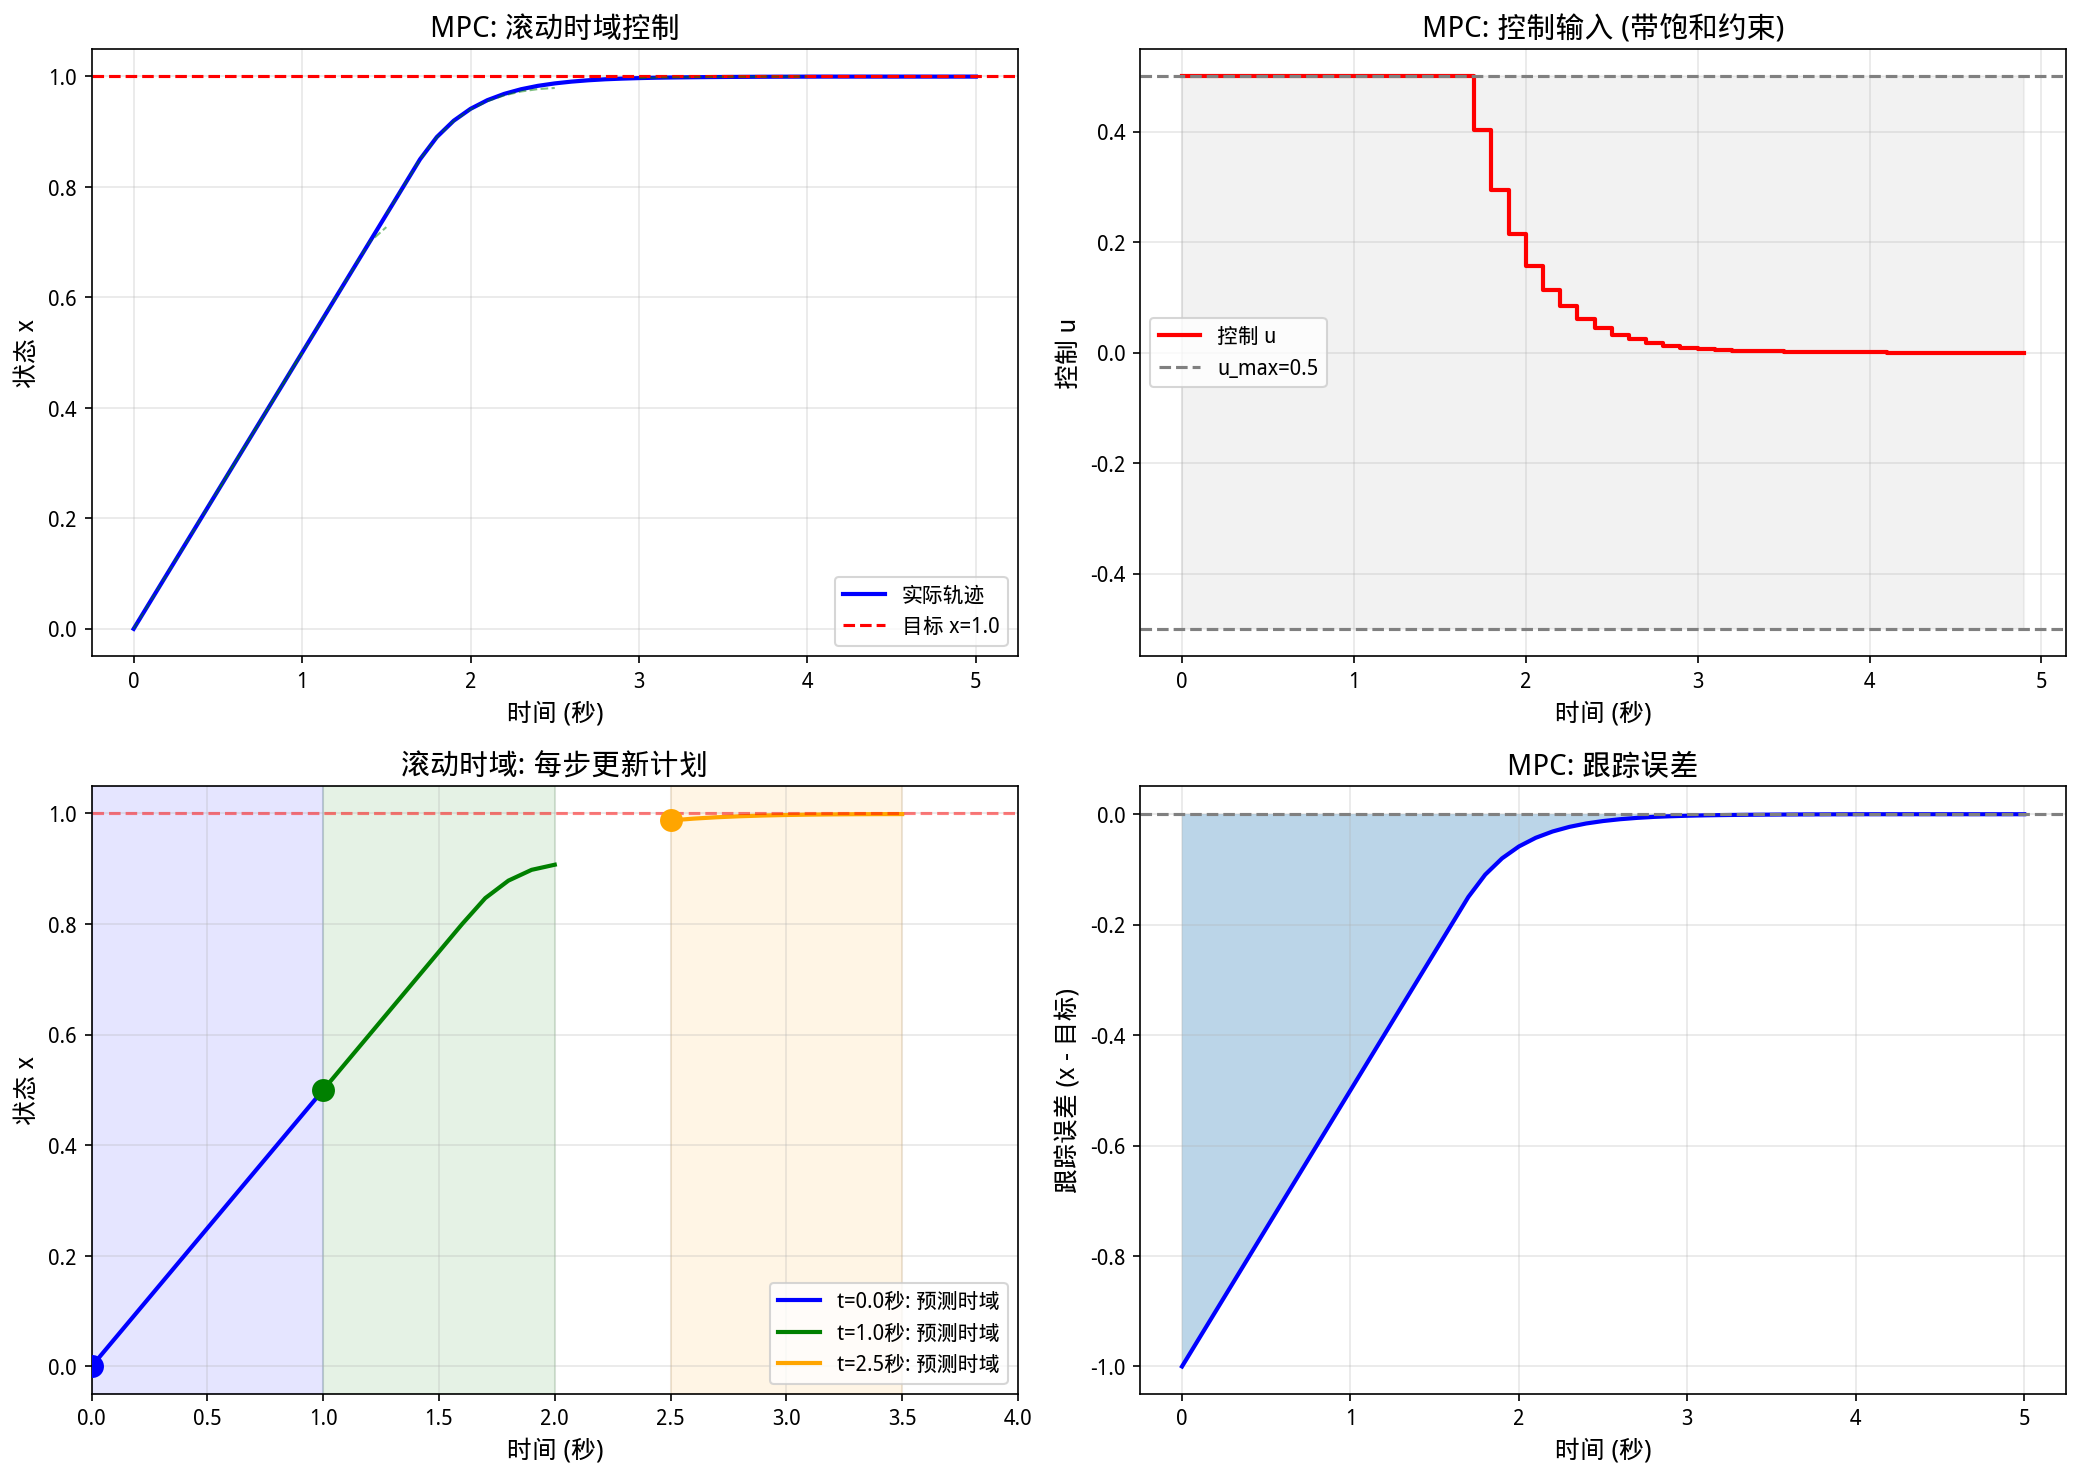
\includegraphics[width=0.98\textwidth]{figs_chap08/chap08_fig2.png}
\caption{MPC（模型预测控制）滚动时域演示。左上：实际轨迹与多条预测轨迹——每个时刻重新规划，但只执行第一步；右上：控制输入（饱和在$\pm 0.5$）；左下：滚动时域示意——不同时刻的规划窗口；右下：跟踪误差随时间减小。MPC的核心思想：规划多步但只执行一步，用反馈不断修正。}
\label{fig:chap08_mpc}
\end{figure}

% ------------------------------------------------------------------------------------
\section{本章小结}

\begin{enumerate}
    \item \textbf{轨迹优化}是带微分方程约束的变分问题
    
    \item \textbf{拉格朗日乘子} $\lambda(t)$ 处理动力学约束，物理意义是"未来对现在的影响"
    
    \item \textbf{哈密顿函数} $H = L + \lambda^\top f$ 是拉格朗日函数的连续时间版本
    
    \item \textbf{伴随方程}向后积分，与神经网络的\textbf{反向传播}数学结构相同
    
    \item \textbf{MPC} 是"边走边规划"的策略：规划多步，执行一步，用反馈修正
\end{enumerate}

\begin{unification}[title=统一视角：约束优化无处不在]
\begin{center}
\begin{tabular}{lll}
\toprule
\textbf{问题} & \textbf{约束} & \textbf{乘子的意义} \\
\midrule
静态优化 & $g(x) = 0$ & 约束的"价格" \\
力学系统 & 运动学约束 & 约束力 \\
轨迹优化 & $\dot{x} = f(x, u)$ & 未来代价的敏感度 \\
神经网络 & $z_{k+1} = f(z_k, W_k)$ & 损失对中间层的梯度 \\
\bottomrule
\end{tabular}
\end{center}

从静态到动态，从有限维到无限维，拉格朗日乘子法的思想贯穿始终！
\end{unification}

\begin{physicalmeaning}
\textbf{$\lambda$ 在本章的意义}：$\lambda(t)$ 是动力学约束在时刻 $t$ 的影子价格——"如果此刻有人把状态 $x(t)$ 推开 $\epsilon$，从现在到终点的最小代价会变化 $\lambda(t)^\top \epsilon$"。它有三张面孔：
\begin{itemize}
    \item 往前看第3、4章：把 $L$ 换成拉格朗日量，$\lambda = \partial L/\partial \dot{q}$ 就是广义动量 $p$，伴随方程 $\dot{\lambda} = -\partial H/\partial x$ 就是哈密顿方程 $\dot{p} = -\partial H/\partial q$。
    \item 往后看第9章：把时间步 $k$ 换成网络层 $i$，$\lambda_k$ 就是"误差信号"，伴随方程就是反向传播。
    \item 再往后看第10章：把终点推到无穷远、把代价换成奖励，$\lambda$ 就是值函数的梯度 $\nabla_s V(s)$，伴随方程就变成贝尔曼方程。
\end{itemize}
\end{physicalmeaning}

% ------------------------------------------------------------------------------------
\section{习题}

\paragraph{计算题}
\begin{enumerate}
    \item 对于一维系统 $\dot{x} = u$，最小化 $\int_0^1 u^2 dt$，边界条件 $x(0) = 0$，$x(1) = 1$。
    \begin{enumerate}
        \item 写出哈密顿函数
        \item 写出状态方程、伴随方程、最优性条件
        \item 求解最优控制 $u^*(t)$
        \item 验证 $x^*(t) = t$（匀速运动）
    \end{enumerate}
    
    \item 考虑带终端代价的问题：$\min \int_0^1 \frac{1}{2}u^2 dt + (x(1) - 1)^2$，动力学 $\dot{x} = u$，$x(0) = 0$。
    \begin{enumerate}
        \item 这个问题的终端条件是自由的（不要求 $x(1) = 1$）。推导终端条件 $\lambda(1) = ?$
        \item 求解最优轨迹
    \end{enumerate}
    
    \item （离散化）将问题1离散化为 $N = 4$ 步，用拉格朗日乘子法求解离散最优控制 $u_0^*, u_1^*, u_2^*, u_3^*$。验证与连续解的一致性。
\end{enumerate}

\paragraph{编程题}
\begin{enumerate}
    \setcounter{enumi}{3}
    \item 用直接法数值求解最省力移动问题：把 $\ddot{x} = u$ 离散成 $N = 50$ 步，状态取 $(x_k, v_k)$，用 \texttt{scipy.optimize.minimize}（SLSQP）在等式约束下最小化 $\sum_k u_k^2 \Delta t$。画出 $u_k$，与解析解 $u^*(t) = \frac{6}{T^2}(1 - \frac{2t}{T})$ 比较；打印求解器返回的乘子，验证它们近似等于 $\lambda(t_k)$。
    
    \item 实现本章"小车刹车"的 MPC 控制器：预测时域 $N = 5$，控制受限 $|u_k| \le 3$，每一步只执行 $u_0^*$；在仿真中加入随机扰动（速度每步加上 $\mathcal{N}(0, 0.3^2)$ 的噪声），比较开环控制与 MPC 的轨迹。
\end{enumerate}

\paragraph{思考题}
\begin{enumerate}
    \setcounter{enumi}{5}
    \item 伴随方程为什么要\textbf{向后}积分？这和"未来影响现在"有什么关系？
    
    \item MPC 每步都要求解一个优化问题，计算量很大。有什么方法可以加速？
    
    \item 如果模型不准确（真实动力学和假设的不同），MPC 还能工作吗？为什么？
    
    \item 比较 MPC 和强化学习：
    \begin{itemize}
        \item MPC 需要知道模型 $f(x, u)$，强化学习不需要
        \item MPC 在线计算，强化学习离线训练
        \item 它们各有什么优缺点？
    \end{itemize}
    \preview{第10章会正面回答这道题：强化学习的值函数 $V(s)$ 就是本章的乘子（对所有状态预先算好的 $\lambda$），贝尔曼方程就是伴随方程的无限时域版本；MPC 与强化学习的差别，是"在线解 $\lambda$"还是"离线学 $V$"。}
\end{enumerate}

\paragraph{拓展题}
\begin{enumerate}
    \setcounter{enumi}{9}
    \item （倒立摆）倒立摆的动力学是非线性的。查阅资料，了解如何用线性化 + MPC 控制倒立摆。
    
    \item （Neural ODE）了解"神经常微分方程"的概念。它如何把神经网络和常微分方程统一起来？
\end{enumerate}

% ====================================================================================
\section*{扩展阅读：约束、投影与"能不能到达"的问题}
\addcontentsline{toc}{section}{扩展阅读：约束、投影与"能不能到达"的问题}
% ====================================================================================

在本章中，我们学习了轨迹优化：给定起点和终点，找最优路径。但有一个更基本的问题我们还没问：

\textbf{这条路径存在吗？从 $A$ 出发，我们能不能到达 $B$？}

这就是\textbf{能控性}（controllability）问题。

让我们从一个生活中的例子开始。

%------------------------------------------------------------------------------
\subsection*{一个停车问题}
%------------------------------------------------------------------------------

假设你要把车停进一个平行车位。

\begin{figure}[htbp]
\centering
\begin{tikzpicture}[scale=0.85]
    % 停车位
    \fill[gray!20] (4, -0.5) rectangle (7, 1.5);
    \draw[thick] (4, -0.5) -- (4, 1.5);
    \draw[thick] (7, -0.5) -- (7, 1.5);
    \node at (5.5, 0.5) {\small 车位};
    
    % 初始位置的车
    \begin{scope}[shift={(1, 2)}, rotate=0]
        \draw[thick, fill=blue!30] (-0.6, -0.3) rectangle (0.6, 0.3);
        \fill (0.4, 0.25) circle (1.5pt);
        \fill (0.4, -0.25) circle (1.5pt);
        \fill (-0.4, 0.25) circle (1.5pt);
        \fill (-0.4, -0.25) circle (1.5pt);
    \end{scope}
    \node[blue] at (1, 2.8) {\small 你的车};
    
    % 目标位置的车（虚线）
    \begin{scope}[shift={(5.5, 0.5)}, rotate=0]
        \draw[thick, dashed, red] (-0.6, -0.3) rectangle (0.6, 0.3);
    \end{scope}
    \node[red] at (5.5, -0.3) {\small 目标};
    
    % 问号
    \node[font=\Large] at (3, 1.5) {?};
\end{tikzpicture}
\caption{平行泊车：怎么把车停进去？}
\end{figure}

你有两个控制：
\begin{itemize}
    \item 油门/刹车：控制前进或后退
    \item 方向盘：控制转向
\end{itemize}

\textbf{关键观察}：车不能横着走！

你没法让车直接"平移"进车位。但是，通过前进、后退、转向的组合，你确实可以把车停进去。

\textbf{问题}：为什么两个控制（油门和方向盘）可以让车在三维空间（位置 $x, y$ 和朝向 $\theta$）中自由移动？

答案和我们熟悉的\textbf{约束优化}有深刻的联系。

%------------------------------------------------------------------------------
\subsection*{从约束优化说起}
%------------------------------------------------------------------------------

让我们回顾一下约束优化的核心思想。

\paragraph{等式约束下的优化}

考虑问题：
\begin{equation}
\min f(x) \quad \text{s.t.} \quad g(x) = 0
\end{equation}

约束 $g(x) = 0$ 把我们限制在一个曲面上。在这个曲面上，我们不能朝任意方向走——只能沿着曲面的\textbf{切方向}走。

\begin{figure}[htbp]
\centering
\begin{tikzpicture}[scale=1.0]
    % 曲面（简化为曲线）
    \draw[thick, blue] plot[smooth, domain=-2:2] (\x, {0.3*\x*\x});
    \node[blue] at (2.5, 1.2) {约束曲面};
    
    % 当前点
    \fill[red] (1, 0.3) circle (3pt);
    \node[red, above right] at (1, 0.3) {$x$};
    
    % 切方向（可行）
    \draw[->, green!60!black, very thick] (1, 0.3) -- (2, 0.9);
    \node[green!60!black, right] at (2, 0.9) {切方向（可行）};
    
    % 法方向（不可行）
    \draw[->, gray, thick, dashed] (1, 0.3) -- (1, 1.3);
    \node[gray, right] at (1, 1.3) {法方向（不可行）};
    
    % 梯度
    \draw[->, orange, thick] (1, 0.3) -- (0.4, 0.9);
    \node[orange, left] at (0.4, 0.9) {$\nabla g$};
\end{tikzpicture}
\caption{约束曲面上，只能沿切方向移动}
\end{figure}

\paragraph{可行方向}

在点 $x$ 处，\textbf{可行方向}是满足以下条件的方向 $v$：
\begin{equation}
\nabla g(x)^\top v = 0
\end{equation}

也就是说，$v$ 必须垂直于约束的梯度 $\nabla g$——这样才能保持在约束曲面上。

所有可行方向构成一个\textbf{子空间}——约束曲面的\textbf{切空间}。

\paragraph{投影的视角}

如果我们想朝某个方向 $d$ 走，但 $d$ 不是可行方向怎么办？

答案是：把 $d$ \textbf{投影}到切空间上！

\begin{equation}
d_{\text{可行}} = d - \frac{\nabla g^\top d}{\|\nabla g\|^2} \nabla g
\end{equation}

这就是\textbf{投影梯度法}的核心思想：先计算梯度，再投影到可行方向上。

%------------------------------------------------------------------------------
\subsection*{控制系统中的"约束"}
%------------------------------------------------------------------------------

现在让我们把这个思想用到控制系统上。

\paragraph{汽车的运动学}

汽车的状态是 $(x, y, \theta)$：位置和朝向。

运动方程：
\begin{align}
\dot{x} &= v \cos\theta \\
\dot{y} &= v \sin\theta \\
\dot{\theta} &= \omega
\end{align}

其中 $v$ 是速度（前进/后退），$\omega$ 是转向角速度。

\paragraph{瞬时可达方向}

在任意状态 $(x, y, \theta)$，通过选择 $v$ 和 $\omega$，状态的变化率 $(\dot{x}, \dot{y}, \dot{\theta})$ 可以是：

\begin{equation}
\begin{pmatrix} \dot{x} \\ \dot{y} \\ \dot{\theta} \end{pmatrix} = 
v \underbrace{\begin{pmatrix} \cos\theta \\ \sin\theta \\ 0 \end{pmatrix}}_{g_1} + 
\omega \underbrace{\begin{pmatrix} 0 \\ 0 \\ 1 \end{pmatrix}}_{g_2}
\end{equation}

这意味着：瞬时可达的方向是 $g_1$ 和 $g_2$ 的\textbf{线性组合}。

\paragraph{问题来了}

$g_1$ 和 $g_2$ 只张成一个\textbf{二维}子空间！

但状态空间是三维的 $(x, y, \theta)$。

\textbf{缺失的方向是什么？}

\begin{itemize}
    \item $g_1 = (\cos\theta, \sin\theta, 0)$：沿车身方向（前进/后退）
    \item $g_2 = (0, 0, 1)$：原地转向
\end{itemize}

缺失的是：$(\sin\theta, -\cos\theta, 0)$——\textbf{垂直于车身的方向}（横向移动）！

\begin{figure}[htbp]
\centering
\begin{tikzpicture}[scale=1.1]
    % 三维坐标系
    \draw[->] (0, 0) -- (4, 0) node[right] {$x$};
    \draw[->] (0, 0) -- (0, 3) node[above] {$y$};
    \draw[->] (0, 0) -- (-1.5, -1) node[below left] {$\theta$};
    
    % 车的位置（在 xy 平面上）
    \begin{scope}[shift={(2, 1.5)}]
        % 车身（朝向约30度）
        \draw[thick, fill=gray!30, rotate=30] (-0.4, -0.2) rectangle (0.4, 0.2);
        
        % g1: 前进方向（在xy平面内）
        \draw[->, blue, very thick, rotate=30] (0, 0) -- (1.2, 0);
        \node[blue, rotate=30] at (1.1, 0.5) {$g_1$};
        \node[blue, font=\small] at (2.2, 1.8) {前进/后退};
        
        % 缺失的方向（垂直于车身，在xy平面内）
        \draw[->, red, very thick, dashed, rotate=30] (0, 0) -- (0, -1);
        \node[red, font=\small] at (1.8, -0.2) {缺失！};
        \node[red, font=\small] at (2.8, -0.5) {（横向移动）};
    \end{scope}
    
    % g2: 转向（沿theta轴）
    \draw[->, green!60!black, very thick] (2, 1.5) -- (1, 0.8);
    \node[green!60!black] at (0.5, 1.3) {$g_2$};
    \node[green!60!black, font=\small] at (0.3, 0.7) {转向};
    
    % 说明g1和g2张成的平面
    \fill[blue!10, opacity=0.5] (2, 1.5) -- (3.5, 2.1) -- (2.5, 1.1) -- (1, 0.8) -- cycle;
    \node[font=\small] at (3.8, 0.5) {$g_1, g_2$ 张成的};
    \node[font=\small] at (3.8, 0.1) {二维子空间};
    
    % 标注状态空间是三维
    \draw[<->, thick, purple] (5, 0) -- (5, 2.5);
    \node[purple, font=\small, align=center] at (5.8, 1.25) {状态空间\\是三维的};
\end{tikzpicture}
\caption{$g_1$（前进）和 $g_2$（转向）只张成二维子空间，缺失了横向移动的方向}
\end{figure}

这就是为什么车不能直接横着走。

%------------------------------------------------------------------------------
\subsection*{关键问题：怎么产生新方向？}
%------------------------------------------------------------------------------

虽然不能\textbf{瞬时}横移，但能不能通过某种\textbf{组合操作}实现横移呢？

\paragraph{一个思想实验}

想象以下操作（每步走很小的距离 $\epsilon$）：

\begin{enumerate}
    \item 前进一点点
    \item 左转一点点
    \item 后退一点点
    \item 右转一点点（回到原来的朝向）
\end{enumerate}

如果每步都是"直线运动"，走完一圈应该回到原点。

但实际上呢？

\begin{figure}[htbp]
\centering
\begin{tikzpicture}[scale=1.8]
    % 起点
    \fill (0, 0) circle (2pt);
    \node[below] at (0, 0) {起点};
    
    % 第一步：前进（车朝右）
    \draw[->, blue, thick] (0, 0) -- (0.8, 0);
    \node[blue, above] at (0.4, 0) {\small 1. 前进};
    
    % 第二步：左转（车现在朝上）+ 由于在新位置，"前进"方向变了
    \draw[->, red, thick] (0.8, 0) -- (0.8, 0.6);
    \node[red, right] at (0.8, 0.3) {\small 2. 转+走};
    
    % 第三步：后退
    \draw[->, blue, thick, dashed] (0.8, 0.6) -- (0.1, 0.6);
    \node[blue, above] at (0.45, 0.6) {\small 3. 后退};
    
    % 第四步：右转回来
    \draw[->, red, thick, dashed] (0.1, 0.6) -- (0.1, 0.15);
    \node[red, left] at (0.1, 0.35) {\small 4. 转回};
    
    % 净位移
    \draw[->, green!60!black, very thick] (0, 0) -- (0.1, 0.15);
    \node[green!60!black, below right] at (0.05, 0.08) {净位移！};
    
    % 说明
    \node[align=left] at (2.5, 0.3) {走了一圈\\没回到原点！};
\end{tikzpicture}
\caption{前进—转向—后退—转回：产生了横向位移}
\end{figure}

\textbf{惊喜}：走完一圈，车不在原来的位置！产生了一个\textbf{横向的净位移}。

这就是平行泊车的秘密：虽然不能直接横移，但通过"绕圈"可以\textbf{间接}实现横移。

\paragraph{数学推导：为什么会有净位移？}

让我们用微分方程来严格计算。设初始状态为 $(x_0, y_0, \theta_0) = (0, 0, 0)$（在原点，朝右）。

\textbf{第1步：前进 $\epsilon$}

控制 $v = 1, \omega = 0$，持续时间 $\epsilon$：
\begin{align}
x_1 &= x_0 + \epsilon \cos\theta_0 = 0 + \epsilon \cdot 1 = \epsilon \\
y_1 &= y_0 + \epsilon \sin\theta_0 = 0 + \epsilon \cdot 0 = 0 \\
\theta_1 &= \theta_0 = 0
\end{align}

状态变为 $(\epsilon, 0, 0)$。

\textbf{第2步：左转 $\epsilon$}

控制 $v = 0, \omega = 1$，持续时间 $\epsilon$：
\begin{align}
x_2 &= x_1 = \epsilon \\
y_2 &= y_1 = 0 \\
\theta_2 &= \theta_1 + \epsilon = \epsilon
\end{align}

状态变为 $(\epsilon, 0, \epsilon)$。注意：车现在朝向改变了！

\textbf{第3步：后退 $\epsilon$}

控制 $v = -1, \omega = 0$，持续时间 $\epsilon$。

\textbf{关键}：现在 $\theta = \epsilon \neq 0$，所以"后退"的方向变了！
\begin{align}
x_3 &= x_2 - \epsilon \cos\theta_2 = \epsilon - \epsilon \cos\epsilon \\
y_3 &= y_2 - \epsilon \sin\theta_2 = 0 - \epsilon \sin\epsilon \\
\theta_3 &= \theta_2 = \epsilon
\end{align}

用泰勒展开（$\epsilon$ 很小）：$\cos\epsilon \approx 1 - \frac{\epsilon^2}{2}$，$\sin\epsilon \approx \epsilon$
\begin{align}
x_3 &\approx \epsilon - \epsilon(1 - \frac{\epsilon^2}{2}) = \frac{\epsilon^3}{2} \\
y_3 &\approx -\epsilon \cdot \epsilon = -\epsilon^2
\end{align}

\textbf{第4步：右转 $\epsilon$}

控制 $v = 0, \omega = -1$，持续时间 $\epsilon$：
\begin{align}
x_4 &= x_3 \approx \frac{\epsilon^3}{2} \\
y_4 &= y_3 \approx -\epsilon^2 \\
\theta_4 &= \theta_3 - \epsilon = 0
\end{align}

\textbf{最终结果}：
\begin{equation}
\boxed{(x_4, y_4, \theta_4) \approx \left(\frac{\epsilon^3}{2}, -\epsilon^2, 0\right)}
\end{equation}

\textbf{分析}：
\begin{itemize}
    \item $\theta$ 回到了 0（朝向恢复）
    \item $x$ 方向有 $O(\epsilon^3)$ 的小位移（可忽略）
    \item $y$ 方向有 $\boxed{-\epsilon^2}$ 的位移——这就是\textbf{横向净位移}！
\end{itemize}

虽然每一步都只能沿 $g_1$ 或 $g_2$ 方向走，但四步组合下来，产生了一个沿"缺失方向"（$-y$ 方向，即 $[g_1, g_2]$ 方向）的净位移，大小正比于 $\epsilon^2$。

%------------------------------------------------------------------------------
\subsection*{数学描述：李括号}
%------------------------------------------------------------------------------

刚才的"绕圈产生新方向"现象，数学上用\textbf{李括号}（Lie bracket）来描述。

\paragraph{定义}

给定两个向量场 $f$ 和 $g$，它们的李括号 $[f, g]$ 定义为：

\begin{equation}
[f, g] = \frac{\partial g}{\partial x} f - \frac{\partial f}{\partial x} g
\end{equation}

这里 $\frac{\partial f}{\partial x}$ 是 $f$ 的雅可比矩阵（就是我们熟悉的多元函数求导）。

\paragraph{几何意义}

$[f, g]$ 正是"沿 $f$ 走一点、沿 $g$ 走一点、沿 $-f$ 走回来、沿 $-g$ 走回来"产生的\textbf{净位移方向}。

更精确地：如果每步走 $\epsilon$，净位移大约是 $\epsilon^2 \cdot [f, g]$。

\paragraph{为什么会有净位移？}

关键在于：向量场 $f$ 和 $g$ 是\textbf{随位置变化}的！

在不同位置，$f$ 指向不同方向。所以"前进"和"后退"不是简单的互相抵消——在不同位置执行，效果不完全相反。

这就像在地球上走路：从北京向东走1000公里，再向北走1000公里，再向西走1000公里，再向南走1000公里——你不会回到北京！因为地球是弯的，"东"和"西"的方向随位置而变。

%------------------------------------------------------------------------------
\subsection*{手算汽车的李括号}
%------------------------------------------------------------------------------

让我们来算一下汽车系统的 $[g_1, g_2]$。

\paragraph{两个向量场}

\begin{equation}
g_1 = \begin{pmatrix} \cos\theta \\ \sin\theta \\ 0 \end{pmatrix}, \quad
g_2 = \begin{pmatrix} 0 \\ 0 \\ 1 \end{pmatrix}
\end{equation}

\paragraph{计算雅可比矩阵}

$g_1$ 对 $(x, y, \theta)$ 的偏导：
\begin{equation}
\frac{\partial g_1}{\partial (x, y, \theta)} = \begin{pmatrix} 
\frac{\partial (\cos\theta)}{\partial x} & \frac{\partial (\cos\theta)}{\partial y} & \frac{\partial (\cos\theta)}{\partial \theta} \\
\frac{\partial (\sin\theta)}{\partial x} & \frac{\partial (\sin\theta)}{\partial y} & \frac{\partial (\sin\theta)}{\partial \theta} \\
0 & 0 & 0
\end{pmatrix} = \begin{pmatrix} 0 & 0 & -\sin\theta \\ 0 & 0 & \cos\theta \\ 0 & 0 & 0 \end{pmatrix}
\end{equation}

$g_2$ 是常向量（不依赖于 $x, y, \theta$），所以：
\begin{equation}
\frac{\partial g_2}{\partial (x, y, \theta)} = \begin{pmatrix} 0 & 0 & 0 \\ 0 & 0 & 0 \\ 0 & 0 & 0 \end{pmatrix}
\end{equation}

\paragraph{计算李括号}

\begin{align}
[g_1, g_2] &= \frac{\partial g_2}{\partial x} g_1 - \frac{\partial g_1}{\partial x} g_2 \\
&= \mathbf{0} - \begin{pmatrix} 0 & 0 & -\sin\theta \\ 0 & 0 & \cos\theta \\ 0 & 0 & 0 \end{pmatrix} \begin{pmatrix} 0 \\ 0 \\ 1 \end{pmatrix} \\
&= -\begin{pmatrix} -\sin\theta \\ \cos\theta \\ 0 \end{pmatrix} \\
&= \begin{pmatrix} \sin\theta \\ -\cos\theta \\ 0 \end{pmatrix}
\end{align}

\paragraph{这个结果是什么？}

$[g_1, g_2] = (\sin\theta, -\cos\theta, 0)$

这正是\textbf{垂直于车身}的方向！

\begin{figure}[htbp]
\centering
\begin{tikzpicture}[scale=1.3]
    % 车（朝向 theta = 30度）
    \begin{scope}[rotate=30]
        \draw[thick, fill=gray!20] (-0.8, -0.35) rectangle (0.8, 0.35);
        % 前轮
        \fill (0.5, 0.3) circle (2pt);
        \fill (0.5, -0.3) circle (2pt);
    \end{scope}
    
    % g1: 前进方向
    \draw[->, blue, very thick, rotate=30] (0, 0) -- (1.5, 0);
    \node[blue] at (1.8, 0.6) {$g_1$（前进）};
    
    % g2: 转向（绕原点）
    \draw[->, red, very thick] (0.3, 0.5) arc (60:120:0.6);
    \node[red] at (-0.3, 0.9) {$g_2$（转向）};
    
    % [g1, g2]: 横移方向
    \draw[->, green!60!black, very thick, rotate=30] (0, 0) -- (0, -1.2);
    \node[green!60!black] at (0.9, -1.1) {$[g_1, g_2]$（横移）};
    
    % 坐标系
    \draw[->] (-1.5, -1.5) -- (-0.5, -1.5) node[right] {\small $x$};
    \draw[->] (-1.5, -1.5) -- (-1.5, -0.5) node[above] {\small $y$};
\end{tikzpicture}
\caption{汽车的三个方向：$g_1$、$g_2$ 和它们的李括号 $[g_1, g_2]$}
\end{figure}

%------------------------------------------------------------------------------
\subsection*{能控性：什么时候能到达任意位置？}
%------------------------------------------------------------------------------

现在我们可以回答最初的问题了。

\paragraph{可达方向的集合}

汽车有三个"可达方向"：
\begin{itemize}
    \item $g_1$：直接可达（前进/后退）
    \item $g_2$：直接可达（转向）
    \item $[g_1, g_2]$：间接可达（通过"绕圈"实现横移）
\end{itemize}

\paragraph{检验线性无关性}

这三个向量是否线性无关？把它们排成矩阵，计算行列式：

\begin{equation}
\det \begin{pmatrix} \cos\theta & 0 & \sin\theta \\ \sin\theta & 0 & -\cos\theta \\ 0 & 1 & 0 \end{pmatrix}
\end{equation}

按第二列展开：
\begin{equation}
= 1 \cdot \det \begin{pmatrix} \cos\theta & \sin\theta \\ \sin\theta & -\cos\theta \end{pmatrix} = 1 \cdot (-\cos^2\theta - \sin^2\theta) = -1 \neq 0
\end{equation}

行列式非零，所以三个向量\textbf{线性无关}！

\paragraph{结论}

$g_1$、$g_2$、$[g_1, g_2]$ 张成整个三维空间。

这意味着：汽车可以到达状态空间中的\textbf{任意位置}！

虽然只有两个控制输入，但通过巧妙的组合，可以在三维状态空间中自由移动。

%------------------------------------------------------------------------------
\subsection*{与线性代数的联系}
%------------------------------------------------------------------------------

让我们把这个思想和线性代数联系起来。

\paragraph{回顾：线性方程组的解}

考虑 $Ax = b$。什么时候有解？

答案：$b$ 必须在 $A$ 的\textbf{列空间}中。

如果 $A$ 是 $n \times m$ 矩阵，列空间最多是 $m$ 维。只有当列空间充满整个 $\mathbb{R}^n$ 时，任意 $b$ 都有解。

\paragraph{控制系统的类比}

对于控制系统 $\dot{x} = u_1 g_1 + u_2 g_2$：

\begin{itemize}
    \item 瞬时可达方向 = $\text{span}\{g_1, g_2\}$（类比列空间）
    \item 如果 $\text{span}\{g_1, g_2\}$ 不是全空间，有些方向瞬时到不了
\end{itemize}

但控制系统比线性方程组多一个"武器"：\textbf{李括号}！

\begin{center}
\renewcommand{\arraystretch}{1.3}
\begin{tabular}{c|c}
\toprule
\textbf{线性代数} & \textbf{控制系统} \\
\midrule
列空间 $\text{span}\{a_1, \ldots, a_m\}$ & 瞬时可达方向 $\text{span}\{g_1, \ldots, g_m\}$ \\
维数固定 & 可以通过李括号"扩张" \\
$\text{rank}(A) = n$ $\Rightarrow$ 任意 $b$ 有解 & 李代数秩 $= n$ $\Rightarrow$ 能控 \\
\bottomrule
\end{tabular}
\end{center}

\paragraph{控制李代数}

从 $\{g_1, g_2\}$ 出发，不断取李括号，能产生的所有方向构成\textbf{控制李代数}：

\begin{equation}
\mathcal{L} = \text{span}\{g_1, g_2, [g_1, g_2], [g_1, [g_1, g_2]], [g_2, [g_1, g_2]], \ldots\}
\end{equation}

\textbf{能控性判据}：如果 $\dim(\mathcal{L}) = n$（状态空间维数），系统就是能控的。

%------------------------------------------------------------------------------
\subsection*{投影的视角}
%------------------------------------------------------------------------------

让我们从另一个角度理解李括号——\textbf{投影}。

\paragraph{约束优化中的投影}

在约束优化中，我们把梯度投影到可行方向上：

\begin{equation}
\text{可行梯度} = \text{梯度} - \text{（梯度在约束法向上的分量）}
\end{equation}

\paragraph{控制系统中的"约束"是什么？}

汽车的"约束"是：不能横向移动。

数学上，这对应于：
\begin{equation}
\dot{x} \sin\theta - \dot{y} \cos\theta = 0
\end{equation}

（车的横向速度为零）

这是一个\textbf{非完整约束}（nonholonomic constraint）——它约束的是\textbf{速度}，而不是位置。
\review{第7章}{第7章机器人的约束（关节、接触）都是关于位形 $q$ 的约束，可以写成 $g(q) = 0$ 或 $g(q) \ge 0$，叫完整约束。这里"车不能横向滑动"限制的是速度 $\dot{q}$，而且积分不出一个 $g(q) = 0$——这就是"非完整"的含义。}

\paragraph{非完整约束的特殊性}

普通的位置约束（如 $g(x) = 0$）把我们限制在一个曲面上，无论怎么走都逃不出去。

但速度约束不一样！虽然每个瞬间都必须满足约束，但通过巧妙的路径，可以到达"看起来不可达"的位置。

\begin{figure}[htbp]
\centering
\begin{tikzpicture}[scale=0.9]
    % 左边：位置约束
    \begin{scope}
        \node[font=\bfseries] at (2, 3) {位置约束 $g(x, y) = 0$};
        \draw[thick, blue] plot[smooth, domain=-0.5:4.5] (\x, {1 + 0.3*sin(\x r)});
        \fill[red] (1, {1 + 0.3*sin(1 r)}) circle (3pt);
        \fill[gray] (2, 2.5) circle (3pt);
        \node[gray] at (2.5, 2.5) {\small 不可达};
        \node at (2, -0.5) {\small 被困在曲线上};
    \end{scope}
    
    % 右边：速度约束
    \begin{scope}[xshift=7cm]
        \node[font=\bfseries] at (2, 3) {速度约束（非完整）};
        \draw[->] (0, 0) -- (4.5, 0) node[right] {$x$};
        \draw[->] (0, 0) -- (0, 2.8) node[above] {$y$};
        
        % 可达区域（整个平面）
        \fill[green!10] (0.1, 0.1) rectangle (4.3, 2.6);
        
        % 一条曲折的路径
        \draw[red, thick, ->] (1, 0.5) to[out=0, in=-90] (2, 1) to[out=90, in=180] (3, 1.5) to[out=0, in=-90] (3.5, 2);
        
        \fill[red] (1, 0.5) circle (3pt);
        \fill[red] (3.5, 2) circle (3pt);
        
        \node at (2, -0.5) {\small 整个平面可达（绕路）};
    \end{scope}
\end{tikzpicture}
\caption{位置约束 vs 速度约束：后者限制了瞬时方向，但不限制最终位置}
\end{figure}

%------------------------------------------------------------------------------
\subsection*{一个不能控的例子：火车}
%------------------------------------------------------------------------------

为了对比，看一个\textbf{不能控}的系统。

\paragraph{火车模型}

火车只能沿轨道前进/后退：
\begin{equation}
\begin{pmatrix} \dot{x} \\ \dot{y} \end{pmatrix} = v \begin{pmatrix} 1 \\ 0 \end{pmatrix}
\end{equation}

只有一个控制向量场 $g_1 = (1, 0)$。

\paragraph{李括号}

$[g_1, g_1] = 0$（任何向量和自己的李括号都是零，因为"绕圈"回到原点）。

没有其他向量场可以取李括号，所以：
\begin{equation}
\mathcal{L} = \text{span}\{g_1\} = \text{span}\{(1, 0)\}
\end{equation}

维数是1，但状态空间是2维。

\paragraph{结论}

火车不能控！只能沿 $x$ 轴移动，永远到不了 $y \neq 0$ 的位置。

\begin{figure}[htbp]
\centering
\begin{tikzpicture}[scale=0.9]
    % 火车
    \draw[->] (0, 0) -- (5, 0) node[right] {$x$};
    \draw[->] (0, -1) -- (0, 2) node[above] {$y$};
    
    % 轨道
    \draw[brown, line width=3pt] (0, 0) -- (4.5, 0);
    
    % 火车图标
    \draw[thick, fill=gray!30] (2, -0.2) rectangle (3, 0.2);
    \draw[thick] (2.2, 0.2) -- (2.2, 0.4) -- (2.8, 0.4) -- (2.8, 0.2);
    
    % 可达区域
    \draw[green!60!black, very thick, <->] (0.5, 0) -- (4, 0);
    \node[green!60!black, below] at (2.25, -0.4) {\small 可达};
    
    % 不可达
    \fill[red] (3, 1.5) circle (3pt);
    \node[red, right] at (3.1, 1.5) {\small 不可达};
    \draw[red, dashed] (2.5, 0) -- (3, 1.5);
    \node[red] at (2.2, 0.8) {\small ?};
\end{tikzpicture}
\caption{火车只能沿轨道移动，离开轨道的点永远到不了}
\end{figure}

%------------------------------------------------------------------------------
\subsection*{回到线性系统：Kalman 秩条件}
%------------------------------------------------------------------------------

你可能学过线性系统的能控性判据。让我们看看它和李括号的关系。

\paragraph{线性系统}

\begin{equation}
\dot{x} = Ax + Bu
\end{equation}

这可以写成：$\dot{x} = Ax + u_1 b_1 + u_2 b_2 + \cdots$，其中 $b_i$ 是 $B$ 的列向量。

\paragraph{Kalman 秩条件}

线性系统能控的充要条件是：
\begin{equation}
\text{rank}[B \mid AB \mid A^2B \mid \cdots \mid A^{n-1}B] = n
\end{equation}

\paragraph{和李括号的联系}

对于线性系统，漂移项是 $f_0(x) = Ax$，控制向量场是 $g_i = b_i$（$B$ 的列）。

计算李括号：
\begin{equation}
[f_0, g_i] = \frac{\partial g_i}{\partial x} (Ax) - \frac{\partial (Ax)}{\partial x} g_i = 0 - A \cdot b_i = -Ab_i
\end{equation}

继续：
\begin{equation}
[f_0, [f_0, g_i]] = -A(-Ab_i) = A^2 b_i
\end{equation}

所以：

\begin{center}
\renewcommand{\arraystretch}{1.3}
\begin{tabular}{c|c}
\toprule
\textbf{Kalman 矩阵的列} & \textbf{对应的李括号} \\
\midrule
$b_i$ & $g_i$ \\
$Ab_i$ & $-[f_0, g_i]$ \\
$A^2 b_i$ & $[f_0, [f_0, g_i]]$ \\
\bottomrule
\end{tabular}
\end{center}

\textbf{结论}：Kalman 秩条件就是李代数秩条件的线性版本！

%------------------------------------------------------------------------------
\subsection*{本节小结}
%------------------------------------------------------------------------------

\begin{enumerate}
    \item \textbf{能控性}问：从 $A$ 能不能到 $B$？这比"怎么最优地到达"更基本。
    
    \item 控制系统的\textbf{瞬时可达方向}可能不是全空间（比如汽车不能横移）。
    
    \item \textbf{李括号} $[f, g]$ 描述了"绕圈"产生的新方向——这是组合运动的数学描述。
    
    \item \textbf{能控性判据}：控制李代数的维数 = 状态空间维数 $\Rightarrow$ 能控。
    
    \item 汽车虽然只有2个控制，但李括号补上了第3个方向，所以在3维空间中能控。
    
    \item 线性系统的 \textbf{Kalman 秩条件}是李代数秩条件的特例。
\end{enumerate}

\begin{remark}
\textbf{约束优化的统一视角}：

\begin{itemize}
    \item 静态优化：约束 $g(x) = 0$ 限制了可行的\textbf{位置}
    \item 轨迹优化：动力学 $\dot{x} = f(x, u)$ 限制了可行的\textbf{速度}
    \item 能控性：问的是约束是否"太强"——强到无法到达某些状态
\end{itemize}

李括号告诉我们：速度约束有时候比看起来"弱"——通过组合运动可以突破瞬时的限制。

这就像人生：每一步都受限，但正确的组合可以带你到意想不到的地方。
\end{remark}
